\documentclass[10pt]{beamer}

%% ============================================
%% Preámbulo con los paquetes utilizados
\usepackage[spanish]{babel} % Idioma
\usepackage[utf8]{inputenc} % Codificación
\usepackage{pgfpages}
\usepackage{times}
\usepackage[T1]{fontenc}
\usepackage{tikz}
%\usepackage{graphicx}
\usepackage{subcaption}

\usepackage{multimedia}
\usepackage{hyperref}

\setbeamertemplate{footline}[frame number]

\usetheme{CambridgeUS}
\usecolortheme{dolphin}

\setbeamertemplate{sections/subsections in toc}[square]
\setbeamertemplate{itemize items}[square]

%\setbeamercolor{block body alerted}{bg=alerted text.fg!10}
%\setbeamercolor{block title alerted}{bg=alerted text.fg!20}
\setbeamercolor{block body}{bg=structure!10}
\setbeamercolor{block title}{bg=structure!20}
%\setbeamercolor{block body example}{bg=green!10}
%\setbeamercolor{block title example}{bg=green!20}

\AtBeginSection[]{
  \begin{frame}
  \vfill
  \centering
  \begin{beamercolorbox}[sep=8pt,center,shadow=true,rounded=true]{title}
    \usebeamerfont{title}\insertsectionhead\par%
  \end{beamercolorbox}
  \vfill
  \end{frame}
}

%% ============================================
%% Definiciones para la primer diapositiva
%\title{Diseño y Construcción de una Computadora de Vuelo para Vehículos Autónomos con Tolerancia a Fallas}
%\date{COMPLETAR}
%\author[Federico Ignacio Nuñez Frau]{Federico Ignacio Nuñez Frau\\[1ex]  {\small Director: Dr. Ing. Claudio Pose (FIUBA)}\\ {\small Co-Director: Ing. Leonardo Garberoglio (UTN-FRSN)}}
%\author{Federico Ignacio Nuñez Frau (98211)}
%\titlegraphic{\includegraphics[width=0.3\textwidth]{img/logo-fiuba.png}}
% \titlegraphic{
% \begin{tikzpicture}[overlay,remember picture]
% \node[] at (3, 0){
%   \includegraphics[width=0.2\linewidth]{img/logo-fiuba.png}};
%   \end{tikzpicture}
%   }

% \makeatletter
% \setbeamertemplate{title page}[default][left,colsep=-4bp,rounded=true,shadow=\beamer@themerounded@shadow]
% \makeatother

\makeatletter
\newcommand\titlegraphicii[1]{\def\inserttitlegraphicii{#1}}
\titlegraphicii{}
\setbeamertemplate{title page}
{
  \vbox{}
  \begin{centering}
    \begin{beamercolorbox}[sep=8pt,center]{title}
      \usebeamerfont{title}\inserttitle\par%
    \end{beamercolorbox}%
    \vskip1em\par
    \begin{beamercolorbox}[sep=8pt,center]{author}
      \usebeamerfont{author}\insertauthor
    \end{beamercolorbox}
    \begin{beamercolorbox}[sep=8pt,center]{date}
      \usebeamerfont{date}\insertdate
    \end{beamercolorbox}%\vskip0.5em
    {\usebeamercolor[fg]{titlegraphic}\inserttitlegraphic\hfill\inserttitlegraphicii\par}
  \end{centering}
  %\vfill
}
\makeatother
\author[Federico Ignacio Nuñez Frau]{Federico Ignacio Nuñez Frau - 98211\\[1ex]  {\small Director: Dr. Ing. Claudio Pose (FIUBA)}\\ {\small Co-Director: Ing. Leonardo Garberoglio (UTN-FRSN)}}
\title[]{Diseño y Construcción de una Computadora de Vuelo para Vehículos Autónomos con Tolerancia a Fallas}
\date{DD/MM/2024}
\titlegraphic{\includegraphics[width=0.23\linewidth]{img/logo-fiuba.png}}
%\titlegraphicii{\includegraphics[height=1cm,width=2cm]{logo2}}

%% ============================================
%% Comienzo del documento
\begin{document}

%% Carátula
\begin{frame}
  \titlepage
  % \small
  %   Director:\\[0,1cm]
  %   Dr. Ing. Claudio Pose (FIUBA) \\[0.25cm]
  %   Co-Director:\\[0,1cm]
  %   Ing. Leonardo Garberoglio (UTN-FRSN) \\[0.25cm]
\end{frame}

%% Contenidos de la presentación
\begin{frame}{Contenidos}
  \tableofcontents
\end{frame}

% \begin{frame}{Ejemplo de cómo embeber un video}
%   \centering
%   \movie[externalviewer]{\includegraphics[width=\textwidth, keepaspectratio]{img/cavidad.png}}{vid/AON.mp4}
% \end{frame}

\section{Introducción y Motivación}

% ==============================================
\begin{frame}{Vehículos Autónomos}
	\begin{itemize}
		\item <2->Los vehículos autónomos no cuentan con una tripulación ni un piloto a bordo. Estos son comandados de forma remota, o bien tienen la capacidad de hacerlo por sí solos.
		\item <3->Gran variedad de sensores + computadora central = sistema de navegación y reconocimiento del entorno.
	\end{itemize}
	\begin{center}
		\resizebox{\textwidth}{!}{%
			\onslide<4->\includegraphics[height=3cm]{img/uav_2.jpg}%
			\quad
			\onslide<4->\includegraphics[height=3cm]{img/ASV_leo.png}%
			\quad
			\onslide<4->\includegraphics[height=3cm]{img/movil_robot.png}%
		}
	\end{center}
\end{frame}

\begin{frame}{Vehículos Autónomos}
	\begin{columns}
    \column{0.5\textwidth}
        \begin{itemize}
            \item<1->Originalmente desarrollados para uso en aplicaciones militares.
            \item<3->Desarrollo y mantenimiento menos costoso frente a vehículos tripulados.
            \item<4->Motivación: Realizar tareas que de otra forma pondrían en riesgo a la tripulación.
        \end{itemize}
    \column{0.5\textwidth}
            \onslide<2->\includegraphics[width=\textwidth]{img/dron_militar_1}
	\end{columns}
\end{frame}

\begin{frame}{Vehículos Autónomos}
	% \begin{columns}
	% \column{0.5\textwidth}
	%     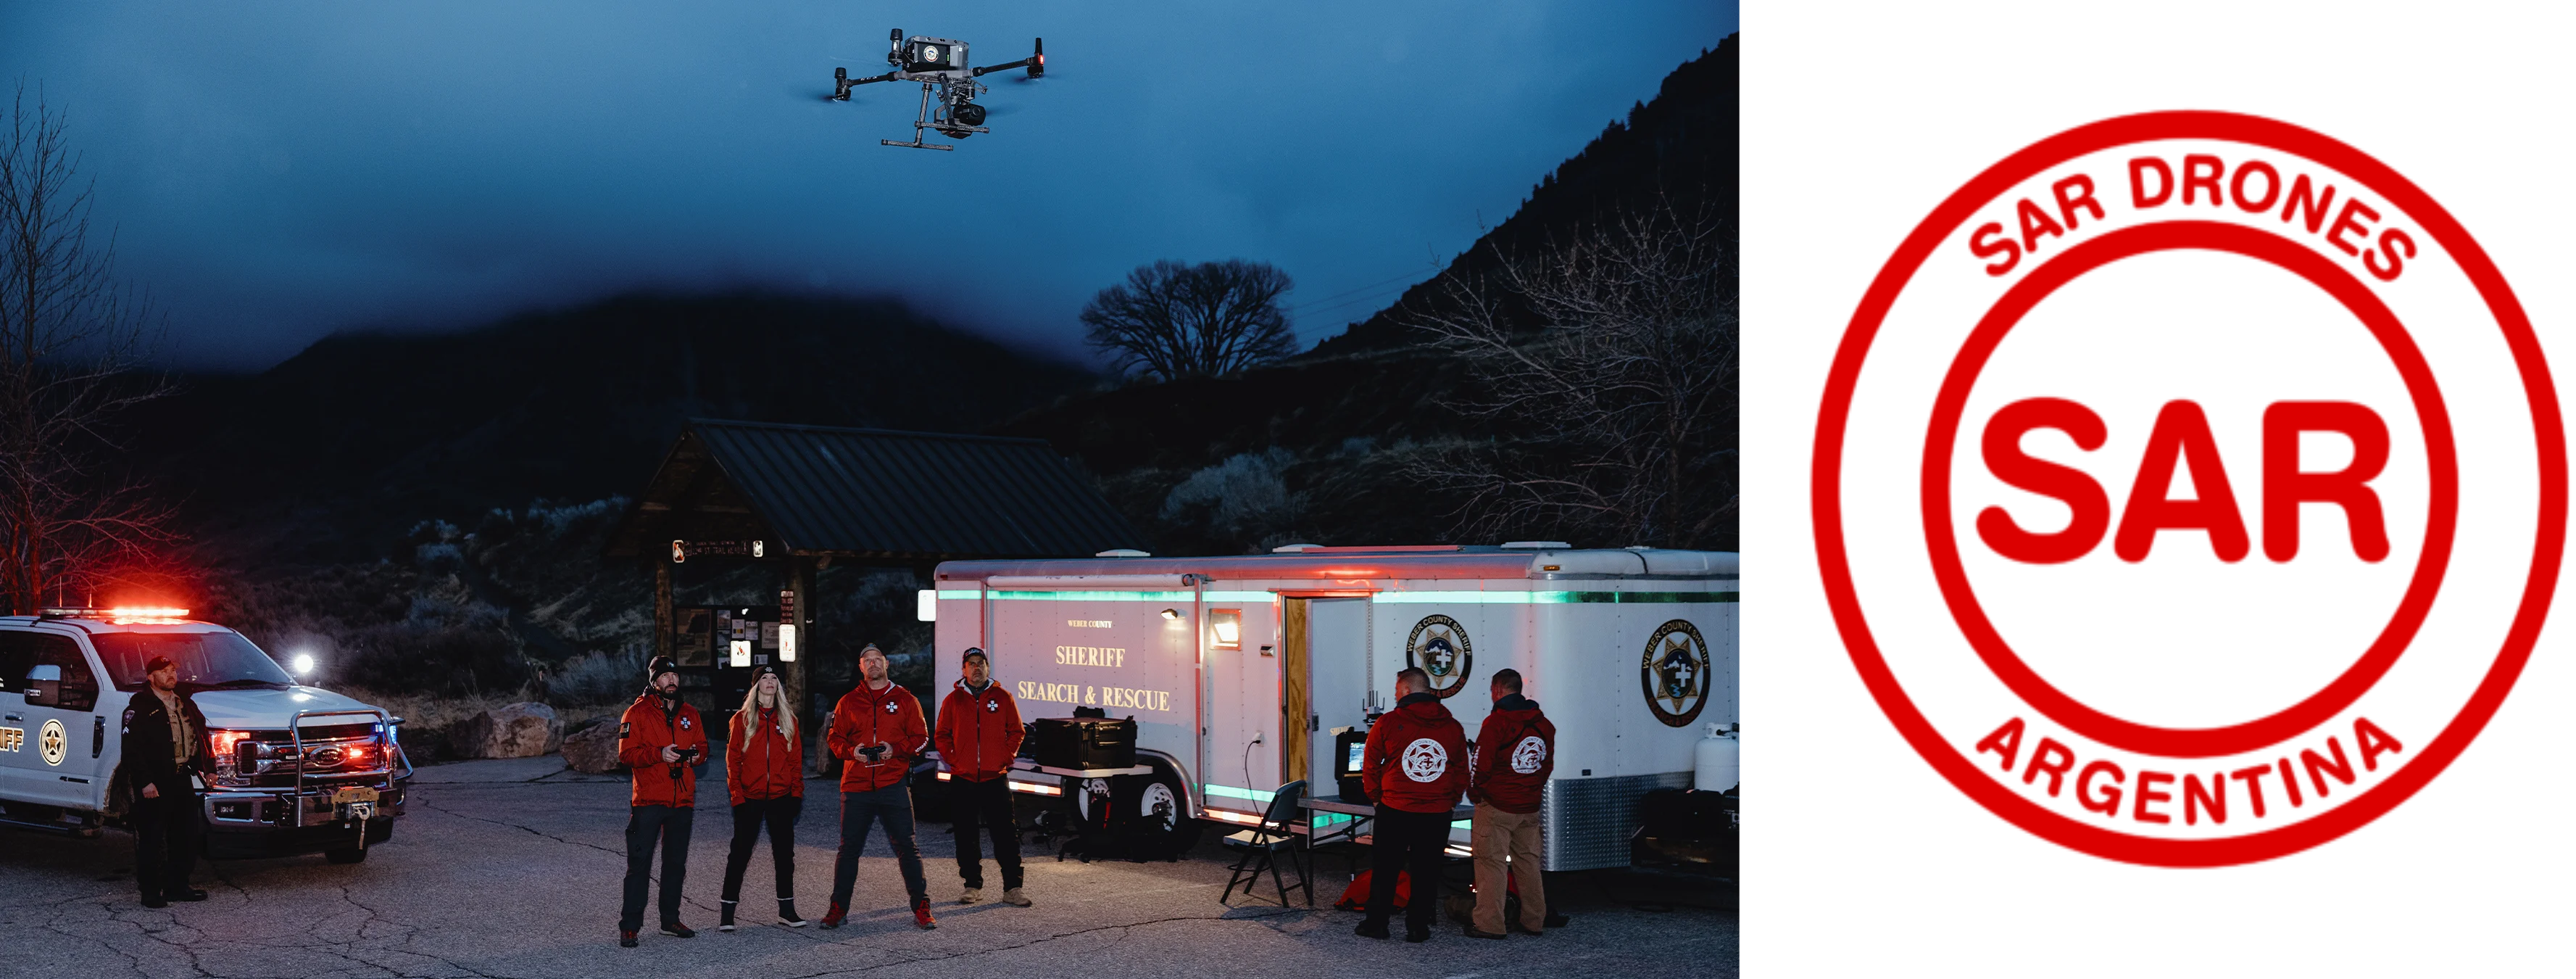
\includegraphics[width=4cm]{img/drones_sar_todo.png}
	%     \includegraphics[width=4cm]{img/drone_camer.png}
	% \column{0.5\textwidth}
	% 	\includegraphics[width=4cm]{img/drone_agricultura.png}
	%     \includegraphics[width=4cm]{img/inspeccion_completo.png}
    % \end{columns}
    % \makebox[\textwidth]{%
	% \begin{minipage}{1\textwidth} % <--- can be as large the slide size permits
	% 	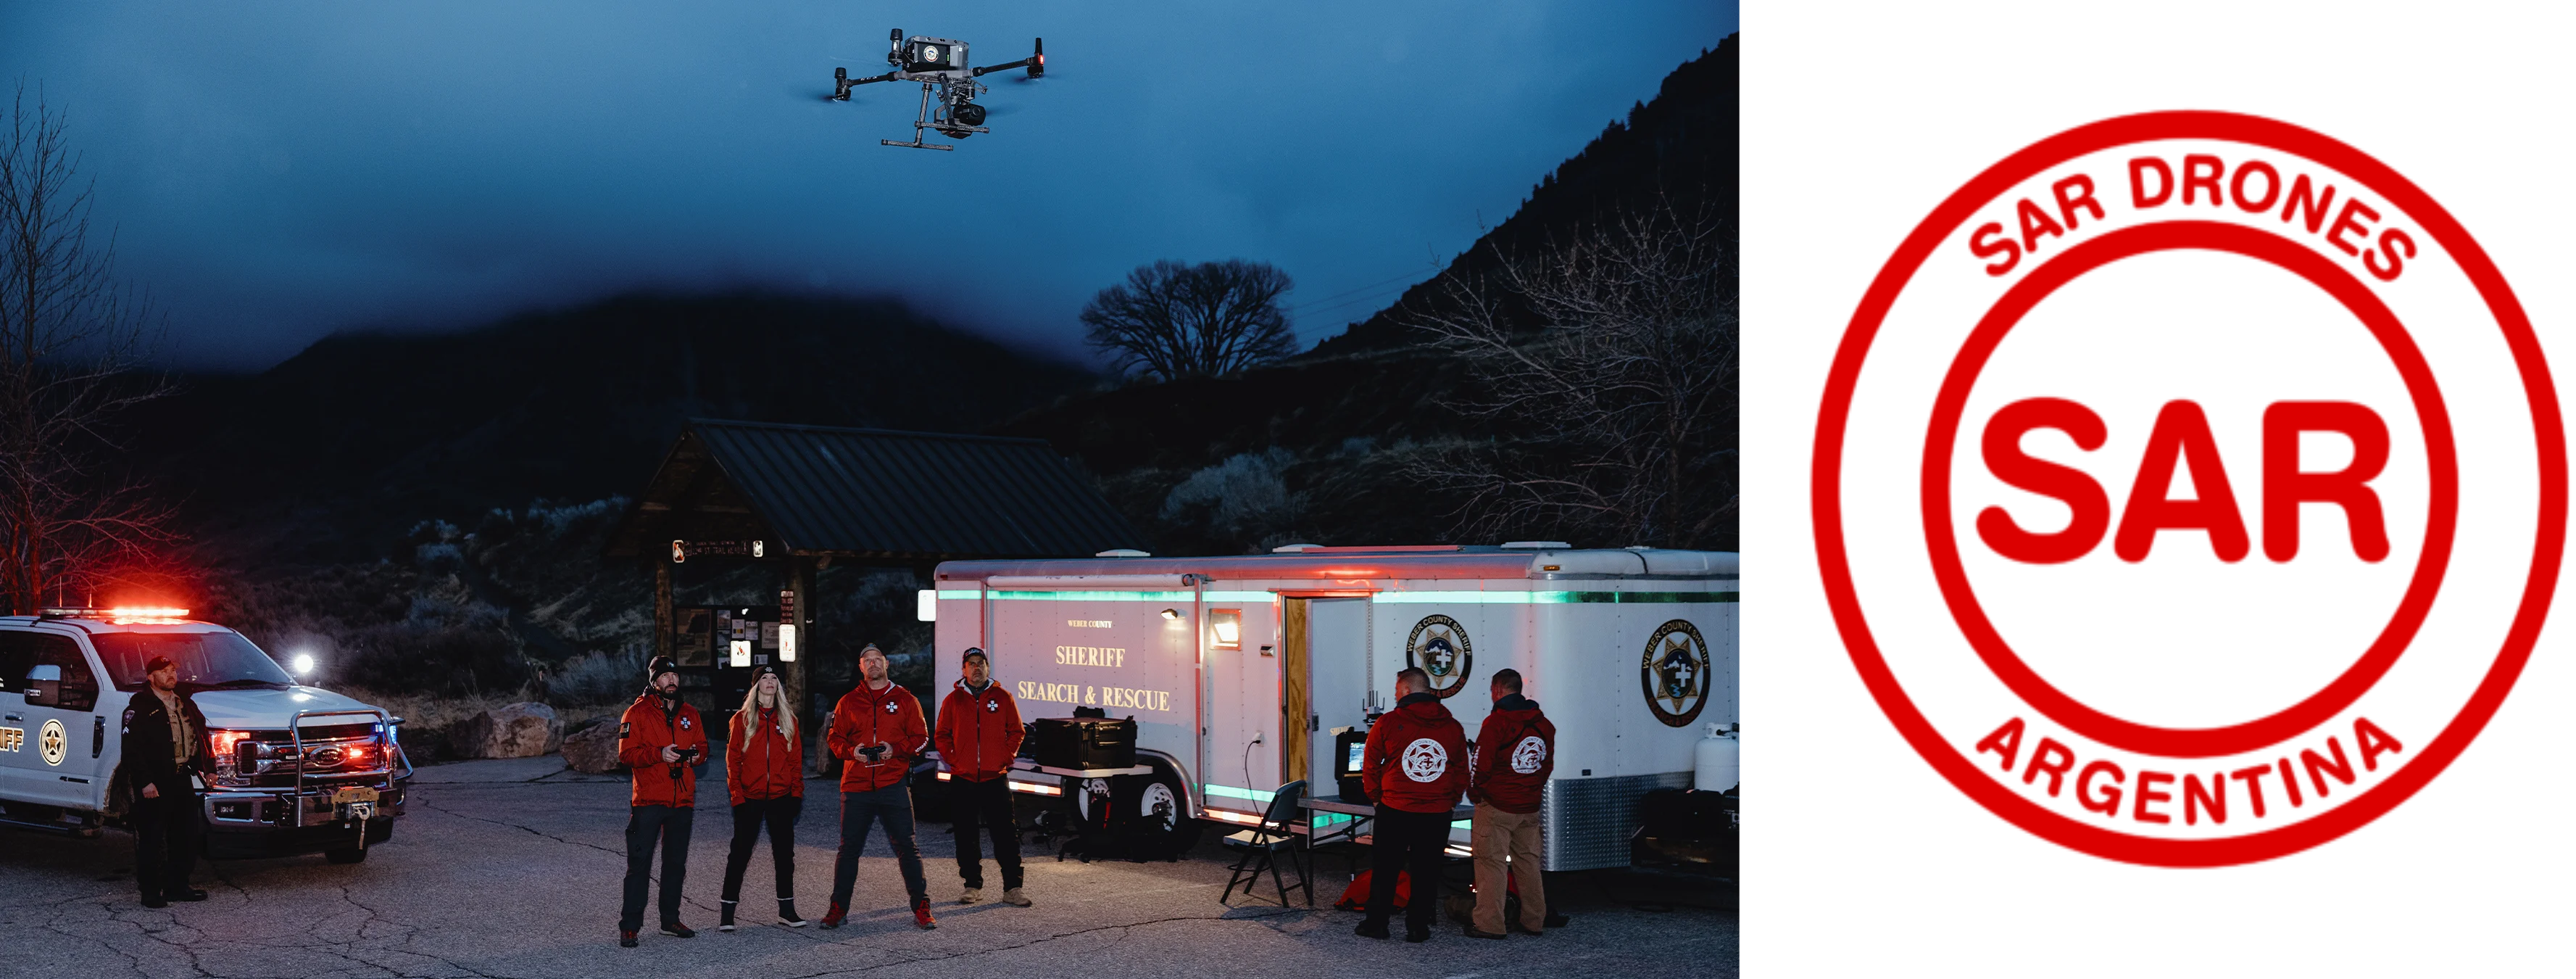
\includegraphics[width=.3\textwidth,keepaspectratio]{img/drones_sar_todo.png}\hfill%
	% 	\includegraphics[width=.3\textwidth,keepaspectratio]{img/drone_camer.png}\\[4pt]
	% 	\includegraphics[width=.3\textwidth,keepaspectratio]{img/inspeccion_completo.png}\hfill%
	% 	\includegraphics[width=.3\textwidth,keepaspectratio]{img/drone_agricultura.png}
	% 	\includegraphics[width=.3\textwidth,keepaspectratio]{img/drone_volcano.png}
	% 	\includegraphics[width=.3\textwidth,keepaspectratio]{img/drone_traffic.png}
	% \end{minipage}
	\makebox[\textwidth]{%
	\begin{minipage}{1\textwidth} % <--- can be as large the slide size permits
		\includegraphics[height=.35\textheight,keepaspectratio]{img/drone_traffic_size.png}\hfill
		\includegraphics[height=.35\textheight,keepaspectratio]{img/drone_volcano_size.png}\hfill
		\includegraphics[height=.35\textheight,keepaspectratio]{img/drone_inspeccion_size.png}\\[20pt]
		\includegraphics[height=.35\textheight,keepaspectratio]{img/drone_agricultura_size.png}\hfill
		\includegraphics[height=.35\textheight,keepaspectratio]{img/drone_camera_size.png}\hfill
		\includegraphics[height=.35\textheight,keepaspectratio]{img/drones_sar_size.png}
	\end{minipage}
}
\end{frame}

\begin{frame}{Vehículos Autónomos}
	\begin{itemize}
		\item<1->Cada vez tienen mayor presencia en zonas civiles.
		\item<2->La incorporación de drones permite realizar tareas costosas,  riesgosas o críticas de forma segura.
		\item<3->Teniendo esto en cuenta, la confiabilidad es un aspecto que toma mayor relevancia.
		\item {COMPLETAR CON EJEMPLOS DE ACCIDENTES DE DRONES}
	\end{itemize}
\end{frame}

% ==============================================
\begin{frame}{Computadora de Vuelo}
	\begin{columns}
		\column{0.39\textwidth}
		\begin{itemize}
			\item <1->Los drones se componen de varios elementos.
			\item <3->Todos ellos son susceptible de manifestar fallas.
			\item <4->En este trabajo se abordan aspectos relacionados a la \textbf{computadora de vuelo}.
		\end{itemize}
		\column{0.6\textwidth}
			\begin{overprint}
				\onslide<2>\includegraphics[width=\textwidth]{img/partes_de_un_drone.png}
				\onslide<3>\includegraphics[width=\textwidth]{img/partes_de_un_drone.png}
				\onslide<4>\includegraphics[width=\textwidth]{img/partes_de_un_drone_transparencia.png}
			\end{overprint}
	\end{columns}
\end{frame}

\begin{frame}{Computadora de Vuelo}
	\begin{columns}
		\column{0.39\textwidth}
			\begin{itemize}
				\item <2->Se encarga de ejecutar los algoritmos de guiado, navegación y control para estabilizar el vehículo y guiarlo en su trayectoria.
				\item <3->Adquiere datos de los sensores del vehículo.
				\item <4->Actúa sobre los motores.
				\item <5->La computadora de vuelo es el elemento central en un vehículo aéreo no tripulado.
			\end{itemize}
		\column{0.6\textwidth}
			\begin{overprint}
				\onslide<2>\includegraphics[width=\textwidth]{img/drone_actuadores_sensores_1.png}
				\onslide<3>\includegraphics[width=\textwidth]{img/drone_actuadores_sensores_2.png}
				\onslide<4>\includegraphics[width=\textwidth]{img/drone_actuadores_sensores.png}
				\onslide<5>\includegraphics[width=\textwidth]{img/drone_actuadores_sensores.png}
			\end{overprint}
	\end{columns}
\end{frame}

% ==============================================
\begin{frame}{Tolerancia a Fallas}
	\begin{itemize}
		\item<1->Cada vez tienen mayor presencia en zonas civiles.
		%\item La incorporación de drones permite realizar tareas costosas,  riesgosas o críticas de forma segura.
		\item<2->Teniendo esto en cuenta, la \textbf{confiabilidad} es un aspecto que toma mayor relevancia.
		\item<3->En vehículos aéreos como aviones comerciales y militares se utilizan técnicas de \textbf{tolerancia a fallas}.
		\item<5->También en drones de uso militar.
	\end{itemize}
    %\begin{block}{Confiabilidad}
    %	Probabilidad de que un sistema pueda cumplir con su función de manera correcta en un intervalo de tiempo $\left[t_0;t\right]$, dado que sí podía hacerlo en $t_0$.
    %\end{block}
    \begin{columns}
    	\column{0.4\textwidth}
			\onslide<4->\includegraphics[width=\textwidth]{img/avion_comercial.jpg}
    	\column{0.6\textwidth}
            \begin{itemize}
            	\item<6->El aspecto más importante en aviones comerciales: $10^{-9}/h$ de vuelo.
            	\item<7->Aviones militares: $10^{-7}/h$ de vuelo.
            	\item<8->Drones militares: $10^{-5}/h$ de vuelo.
            	\item<9->¿\underline{Drones civiles/comerciales}?
            \end{itemize}
    \end{columns}
\end{frame}

% ==============================================
\begin{frame}{Objetivos}
	\begin{enumerate}
		\item \textbf{Estudiar} las características de los sistemas con tolerancia a fallas aplicados en vehículos aéreos, tanto tripulados como no tripulados.
		\item \textbf{Entender} los requerimientos para implementar un sistema con tolerancia a fallas.
		\item \textbf{Diseñar} una computadora de vuelo para vehículos aéreos no tripulados, para ser enviada a fabricar.
		\item \textbf{Desarrollar} un firmware que demuestre la capacidad de ser utilizada en un sistema con tolerancia a fallas.
	\end{enumerate}
\end{frame}

%\section{Análisis de Sistemas Críticos y Tolerancia a Fallas}

\section{Estado del Arte}\label{sec:estado_del_arte}

%En esta sección se analizan distintos casos de implementación de sistemas de control de vuelo redundantes. Si bien en este trabajo se desarrolla una computadora de vuelo para UAVs, se toma como referencia características generales del funcionamiento del sistema utilizado en aviones comerciales, por ser el sistema críticos por excelencia. Estos funcionan correctamente durante muchas horas, trasladando a muchas personas. Seguido a esto, se analizan trabajos y computadoras de vuelo utilizadas en UAVs que implementen redundancias. Los sismteas analizados utilizan distintas técnicas para implenetar las redundancias. Lo que se busca es detectar similitudes y posibles requerimientos que caractericen a un sistema con redundancias. 

En esta sección se analizan distintos casos de vehículos aéreos que utilizan técnicas de tolerancia a fallas a partir de redundancias. Si bien en este trabajo se desarrolla una computadora de vuelo para UAVs, se toman como referencia características generales de sistemas utilizados en aviones comerciales. Estos vehículos tienen requerimientos de confiabilidad extremadamente altos, ya que deben funcionar correctamente durante muchas horas, cargando con la responsabilidad de trasladar de forma segura a muchas personas. 

A su vez, se presentan trabajos y computadoras de vuelo comerciales para UAVs que incluyen redundancias. Lo que se busca es detectar similitudes y posibles requerimientos que caractericen a un sistema que implementa la tolerancia a fallas a partir del uso de redundancias.

\subsection{Redundancias en Sistemas de Control de Vuelo en Aviones}

%En aviónica, el sistema de control de vuelo es sin dudas un sistema crítico.
Los sistemas de control de vuelo en aviones originalmente se encontraban constituidos por sistemas mecánicos muy complejos. Con el pasar de los años estos comenzaron a ser reemplazados por sistemas electrónicos, denominados \textit{fly-by-wire}. Fueron introducidos en vuelos comerciales en el Airbus 320 en 1987 y el Boeing 777 en 1994 \cite{FBWNASA}, con el objetivo de alivianar la carga del avión y mejorar su rendimiento en cuanto al consumo de combustible. Su nombre deriva del hecho de que la acción del piloto no se aplica de manera directa sobre el avión, ya que todas las acciones pasan por un sistema electrónico que se encarga del control de vuelo. Todas las señales de sensores y de comandos son transmitidas eléctricamente desde y hacia una computadora de vuelo.

\begin{figure}[htb]
    \centering
    \includegraphics[width=0.8\textwidth]{img/avion_FBW.png}
    \caption{Esquema simplificado donde se muestran los componentes del sistema de control de vuelo de un avión. Tanto los comandos enviados por el piloto, como los sensores y los actuadores se encuentran conectados a la computadora de vuelo. La imagen se extrajo de \cite{collinson2023introduction}.}
    \label{fig:avion_FBW}
\end{figure}

%{\color{red} La imagen muestra que todo pasa por la computadora de vuelo, incluso los comandos del piloto. Los actuadores y sensores pasan por la computadora de vuelo. En la imagen no se muestran las redundancia}.

En la figura \ref{fig:avion_FBW} se muestran los distintos componentes presentes en un avión y que conforman el sistema \textit{fly-by-wire}. Entre ellos se encuentran los controles del piloto, distintos tipos de sensores, actuadores y la computadora de vuelo. El hecho de que todos los demás componentes se encuentren conectados a esta, deja ver que es el elemento central de todo el sistema. 

Si bien el piloto ejecuta sus comandos a través de accionamientos manuales como pedales, palancas, etc, estos incluyen una electrónica que interpreta los comandos y genera una señal digital, la cual luego es transmitida hacia la computadora de vuelo. Los mismo ocurre en la comunicación con todos los demás componentes, estas se realizan a través de señales digitales.

El avión contiene una serie de sensores de movimiento, como acelerómetros y giróscopos, los cuales son de vital importancia para mantener la estabilidad del vehículo. Las mediciones de estos sensores, junto con los comandos del piloto, son utilizados por la computadra de vuelo para calcular la acción a aplicar sobre los actuadores. Estos luego interpretan esta acción de control recibida y la convierten en una señal analógica, para poder aplicarla sobre la neumática que controla los alerones, el timón, los elevadores y demás accionamientos. %En \cite{yeh1996triple} puede encontrarse una explicación más detallada del funcionamiento de este sistema en el avión Boeing 777.

%A modo de ejemplo en la figura \ref{fig:Boeing_777_diagrama}, se muestra un diagrama simplificado de la arquitectura del sistema de control de vuelo principal del avión Boeing 777. En esta imagen se muestran distintos bloques los cuales se encuentran comunicados a través de un bus. Cuando el piloto del avión quiere ejecutar una acción, este lo hace a través de métodos convencionales como palancas o pedales que se encuentran en la cabina. Estas acciones generan señales analógicas las cuales son entregadas a los bloques denominados \textit{Actuator Control Electronics} (ACEs). Estos bloques convierten la señal analógica en una señal digital que puede enviarse a través del bus de comunicaciones a los bloques denominados \textit{Primary Flight Control System} (PFCs).

% \begin{figure}[H]
%     \centering
%     \includegraphics[width=0.7\textwidth]{img/Boeing_777_diagrama.png}
%     \caption{Arquitectura del sistema principal de vuelo, conformado por varias computadoras en una configuración redundante. La imagen se extrajo de \cite{collinson2023introduction}.}
%     \label{fig:Boeing_777_diagrama}
% \end{figure}

% Además de la acción del piloto, las PFCs toman datos de los distintos sensores para poder calcular todas las acciones de control que se aplicarán a los distintos actuadores del avión. Los resultados de los cálculos son enviados a los actuadores nuevamente a través del bus de comunicación a cada bloque ACE asignado para cada actuador el cual interpreta el comando recibido por el bus y lo convierte en una señal analógica que aplicará su actuador asignado. En \cite{yeh1996triple} puede encontrarse una explicación más detallada del funcionamiento de este sistema en el avión Boeing 777.\\

%En la figura \ref{fig:Boeing_777_diagrama} lo que se observa es que hay redundancias en los bloques PFCs y ACEs. No solo eso, sino que además hay redundancias en el canal de comunicación, es decir en el bus. Por si fuera poco, en el Boeing 777, cada una de las PFCs se compone a su vez de 3 microprocesadores, cada uno con su fuente de alimentación propia e interfaz de comunicación con el bus. Cada uno de esos 3 procesadores son de distintos fabricantes y sus respectivos softwares son desarrollados por grupos de trabajo distintos. Generalmente solo un procesador de cada PFC se encuentra en funcionamiento normal y los otros actúan como monitores, verificando que lo que estas calculan es correcto.

Tanto los sensores, actuadores, accionamientos del piloto, la acomputadora de vuelo y el medio de comunicación entre todos estos cumplen un rol vital en el funcionamiento del sistema de control de vuelo del avión. Para manetener la estabilidad del vehículo y seguir la trayectoria deseada, el sistema continuamente aplica nuevas acciones de control. Para ello debe obtener información de los sensores y de comandos del piloto, calcular una nueva acción y enviarla a los actuadores, de manera periódica. Teniendo en cuenta las consecuencias catastróficas que puede tener el fracaso de cualquiera de estos componentes, resulta necesario garantizar su correcto funcionamiento durante todo el vuelo.

Debido a que en la práctica resulta imposible afirmar que ningún componente del sistema puede presentar fallas, los requerimientos de seguridad se especifican como la probabilidad de fracaso de un sistema. En la bibliografía consultada se indica que el requerimiento para aviones comerciales es sumamente estricto: $10^{-9}/h$ de vuelo \cite[p.~217]{collinson2023introduction} \cite{yeh1996triple} \cite{lala1994architectural}. Para el caso de aviones de uso militar, el requerimiento es unos órdenes de magnitud más laxo: $10^{-7}/h$, debido a que trasladan a menos personas en comparación con aviones comerciales. Estos valores son tan pequeño que resultan prácticamente imposibles de evaluar de forma expermiental, ya que habría que ejecutar el sistema durante $10^9$ horas aproximadamente para observar el fracaso de un avión comercial, y $10^7$ horas para un avión militar.

El hecho de que la probabilidad de falla de los semiconductores no alcance estos valores tan bajos \cite[p.~4]{Fulton2014AirborneEH} impone una limitación prática para el desarrollo de los distintos componentes del sistema de control de vuelo. Para cumplir con el requerimiento de seguridad, se utilizan otras técnicas que involucran redundancias, es decir, el uso de múltiples componentes destinados a la misma funcionalidad. Es por esto que los aviones comerciales incluyen más de una computadra de vuelo para realizar los cálculos involucrados en el sistema de control de vuelo. En la figura \ref{fig:diagrama_general_fly_by_wire} se muestra un diagrama que representa de forma general la comunicación entre los distintos elementos del sistema de control de vuelo, donde se pueden ver múltiples réplicas de sensores, actudaores, computadoras de vuelo y también de los buses de comunicación.

%La probabilidad de falla de los semiconductores no alcanza este valor \cite[p.~272]{kopetz-2011}. Este es el motivo por el cual se incluyen bloques redundantes en los sistemas de control de vuelo. Por ejemplo, el hecho de que cada PFC tenga 3 procesadores de distintos fabricantes permite eliminar problemas que sean propios del componente. A su vez, el hecho de que cada procesador tenga un software distinto desarrollado por un grupo de personas distinto permite que las fallas que estos puedan tener sean eliminadas a tiempo.\\


%Sin dudas todo el sistema de control de vuelo presenta una complejidad muy grande. El hecho de incorporar redundancias en el sistema incrementa notablemente la seguridad. La forma en la que esta se cuantifica es a través de la probabilidad de que el sistema fracase de forma catastrófica. Para aviones comerciales típicamente debe ser $10^{-9}/h$ \cite[p.~217]{collinson2023introduction}. Este valor es tan bajo que incluso es imposible de verificar de forma expermiental, ya que habría que ejecutar el sistema durante $10^9$ horas aproximadamente. La probabilidad de falla de los semiconductores no alcanza este valor \cite[p.~272]{kopetz-2011}. Este es el motivo por el cual se incluyen bloques redundantes en los sistemas de control de vuelo. Por ejemplo, el hecho de que cada PFC tenga 3 procesadores de distintos fabricantes permite eliminar problemas que sean propios del componente. A su vez, el hecho de que cada procesador tenga un software distinto desarrollado por un grupo de personas distinto permite que las fallas que estos puedan tener sean eliminadas a tiempo.\\

%{\color{red} ACÁ AGREGAR UNA CUENTA SÚPER FÁCIL CON UN SISTEMA CON REDUDANCIAS EN PARALELO Y CON LA PROBABILIDAD DE FALLA EXPONENCIAL}.

%El uso de redundancias trae consigo la necesidad de un sistema que administre todas las tareas de manera correcta con el objetivo de cumplir con el nivel de seguridad requerido. Por ejemplo, en el caso del Boeing 777 antes mencionado, detectar cuándo una de las PFCs llegó a un cálculo de la ley de control incorrecto, determinar si un sensor del avión dejó de funcionar y qué acción tomar en cada caso, entre otras.\\

%En la figura \ref{fig:diagrama_general_fly_by_wire} se muestra un diagrama que representa de forma general la comunicación entre los distintos elementos del sistema de control de vuelo. En este se puede ver la redundancia de buses, sensores, actudaores y computadoras de vuelo.

\begin{figure}[htb]
    \centering
    \includegraphics[width=0.8\textwidth]{img/diagrama_general_fly_by_wire.png}
    \caption{Se muestra de manera general las conexiones entre los distintos elementos del sistema de control de vuelo. Tanto los sensores, como los actuadores, los accionamientos del piloto y las computadoras de vuelo presentan redundancias para incrementar el nivel de seguridad. Todas las comunicaciones se llevan a cabo a través de buses de comunicación, los cuales también presentan redundancias. La imagen se extrajo de \cite{collinson2023introduction}.}
    \label{fig:diagrama_general_fly_by_wire}    
\end{figure}

Al tener más de una réplica de cada componente, una falla en alguno de estos no resulta tan crítica, ya que puede utilizarse alguna de las demás como reemplazo. La forma en que se detecta la ocurrencia de una falla es a través de la comparación de resultados entre réplicas, ya que se asume que es muy poco probable que la mayoría de las réplicas presente una falla al mismo tiempo.

\subsubsection{Comparación de Resultados y Tolerancia a Fallas}

Los sensores de movimiento son vitales para mantener la estabilidad del avión. Si cada una de las réplicas funciona adecuadamente, es esperable que los sensores obtengan mediciones muy similares. %De la misma forma, si uno de ellos entrega una medición diferente a la de los otros, se asume que esto ocurrió debido a una falla.
Debido a que estos toman mediciones de variables físicas, como aceleración lineal, velocidad angular, etc, es normal que existan pequeñas diferencias entre réplicas. Esto debe ser tenido en cuenta al momento de realizar las comparaciones, ya que si se permite que estas diferencias sean muy grandes, podría darse por bueno un sensor con fallas. Caso contrario, podría determinarse que un sensor ha fallado, cuando en realidad no fue así. Esto requiere un trabajo de análisis de los sensores para determinar límites aceptables \cite{lala1994architectural}.

%En \cite[p.~221]{collinson2023introduction} se menciona un algoritmo muy simple. Este consiste en tomar una de las mediciones como referencia y comparar las demás contra esta. En la figura \ref{fig:votacion_sensores} se toma el ángulo $\theta_1$ como referencia, ya que $\theta_3 > \theta_1 > \theta_2$. En caso de que la diferencia $| \theta_1 - \theta_2 |$ ó $| \theta_1 - \theta_3 |$ supere un cierto límite, se asume que el sensor presentó una falla. En el caso de la imagen, la diferencia con el sensor 2 es mucho mayor que con el 3 y se asume que este presentó una falla. El valor que se toma como válido es el valor intermedio, $\theta_1$.

Una técnica muy simple consiste en tomar una de las mediciones como referencia y comparar las demás contra esta. En la figura \ref{fig:votacion_sensores} se presenta un ejemplo para el caso de 3 valores, $X_1$, $X_2$ y $X_3$. Se toma el valor $X_1$ como referencia, ya que $X_3 > X_1 > X_2$. En caso de que la diferencia $| X_1 - X_2 |$ ó $| X_1 - X_3 |$ supere un cierto límite, se asume que el sensor presentó una falla. En el caso de la imagen, la diferencia con el sensor 2 es mucho mayor que con el 3 y se asume que este presentó una falla.

\begin{figure}[htb]
    \centering
    \includegraphics[width=0.6\textwidth]{img/votacion_sensores.png}
    \caption{La comparación entre 3 sensores da como resultado que el sensor 2 presentó una falla. En consecuencia deberá tomarse una acción, por ejemplo ignorar al sensor en las próximas iteraciones del lazo de control.}
    \label{fig:votacion_sensores}
\end{figure}

Luego de recolectar los datos de todos los sensores, las computadores de vuelo redundantes proceden a calcular la ley de control para determinar las acciones a aplicar sobre los actuadores. De la misma forma, estas realizan una comparación de los resultados obtenidos. En caso de que cada una utilice un valor distinto de sensor como entrada, luego los resultados a los que llegarán no serán iguales, por más que las 3 computadoras de vuelo se encuentren funcionando correctamente. La presencia de términos integrales en los cálculos de las leyes de control, hará que estas diferencias se incrementen con el pasar del tiempo. Es por esto que en el momento en que se hacen las comparaciones entre los datos de sensores, las computadoras de vuelo deciden por un único valor a utilizar. Para el caso de la figura \ref{fig:votacion_sensores}, se trata del valor de referencia $X_1$. Este método es utilizado en el avión Boeing 777 \cite{yeh1996triple}. 

El mismo procedimiento se repite con los resultados de cálculo de la ley de control. Las computadoras de vuelo deciden por un único resultado y luego lo envían a los actuadores del avión, a través de los buses de comunicación presentes en el avión. Estos permiten la comunicación entre los distintos componentes y las computadoras de vuelo.

%Una vez que se decide por un único valor, se envía la señal de actuación.


%A partir de la comparación se obtiene un único valor el cual es utilizado por el sistema de control. 



%De la misma forma, se realiza una comparación de los resultados del cálculo de la ley de control obtenido por cada una de las computadoras. Una vez que se decide por un único valor, se envía la señal de actuación.

%El mecanismo de tolerancia a fallas es a través de la comparación entre mediciones de sensores y resultados de cálculo de la ley de control. Si todos los sensores redundantes funcionan adecuadamente, es esperable que estos entreguen mediciones muy similares. Por otro lado, si uno de ellos entrega una medición diferente a la de los otros dos, se asume que este presentó una medición incorrecta. Como resultado de la comparación, se obtiene un único valor el cual es utilizado por el sistema de control. De la misma forma, se realiza una comparación de los resultados del cálculo de la ley de control obtenido por cada una de las computadoras. Una vez que se decide por un único valor, se envía la señal de actuación.

%Existen muchos criterios utilizados para seleccionar los valores de sensores. Un aspecto importante a tener en cuenta es que a pesar de que todos los sensores redundantes funcionen adecuadamente, estos presentarán ciertas diferencias en las mediciones, algo que es esperable teniendo en cuenta cuestiones propias de la construcción de cada sensor, ruido, etc. Esto debe ser tenido en cuenta al momento de realizar las comparaciones.

%Este mismo esquema se repite luego del cálculo de la ley de control y de los valores a aplicar sobre cada actuador.

%{\color{red} MENCIONAR LO DEL PAPER DE BOEING 777 QUE HABLA DEL FUNCIONAMIENTO SINCRONIZADO!}.

%El control de vuelo comprende un sistema a lazo cerrado, utilizando comandos del piloto y mediciones de sensores, se calculan las acciones a aplicar sobre los actuadores. Esto se repite periódicamente durante todo el vuelo.

\subsubsection{Bus de Comunicaciones}

Hasta principios de los años 70s, la comunicación entre los distintos módulos dentro de los aviones se realizaba a través de arneses de muchos cables que transmitían información en paralelo. Estos eran tan grandes que podían llegar a pesar cientos de kilogramos. Sumado a esto, la enorme cantidad de cables venía acompañada de muchas conexiones, puntos que son típicos causales de fallas intermitentes. A partir de mediados de los años 70s, se comenzó a implementar el uso de buses de comunicación serial, comunes a todos los módulos del avión. Esto simplificó muchísimo el cableado, además de facilitar el desarrollo de módulos de aviónica, ya que se simplificó la forma de comunicación con el resto del avión.

La comunicación serial a través del bus utiliza un acceso al medio compartido dominado por el tiempo, \textit{time-division multiple acces} (TDMA). Siguiendo con el caso del avión Boeing 777, el protocolo utilizado es el ARINC 629. Este funciona sin un nodo master y permite una conexión de hasta 120 nodos. Solamente uno de ellos puede acceder al medio físico a la vez, lo cual se define por el acceso al medio dominado por el tiempo. El medio de transmisión es un par trenzado, con una velocidad de 2 Mbit/s. A continuación, en la figura \ref{fig:ARINC_629_bus} se muestra el bus ARINC 629.

\begin{figure}[htb]
    \centering
    \includegraphics[width=0.7\textwidth]{img/ARINC_629_bus.png}
    \caption{Se muestra un bus ARINC 629 con 2 nodos conectados. Este consiste en un par trenzado, con terminaciones en los extremos para evitar reflexiones. La conexión de los nodos al bus no es directa si no que se utilizan acopladores. La imagen se extrajo de \cite{yeh1996triple}.}
    \label{fig:ARINC_629_bus}    
\end{figure}

El hecho de que todas las comunicaciones pasen por el mismo bus lo vuelve un punto clave en cuanto a la seguridad, ya que una falla en uno de sus cables dejaría a todos los módulos sin comunicación. Es por esto que se incluyen varios buses de estos en paralelo, como se mostró en la figura \ref{fig:diagrama_general_fly_by_wire}.

Un aspecto a destacar en el bus de comunicaciones es el método de acceso al medio utilizado, TDMA. El envío y recepción de mensajes se implementa por turnos. Este protocolo define en qué instantes de tiempo cada uno de los nodos puede utilizar el medio físico y en cuáles no. Para que no haya colisiones, todos los nodos deben respetar ese timing, el cual se encuentra predefinido. Esto le da determinismo y claridad al comportamiento del bus y del sistema, ya que a priori puede saberse qué mensaje se estará enviando en cada instante de tiempo. Cualquier otro tipo de comportamiento respresentará una falla. Además, al tratarse de un sistema de tiempo real, no pueden permitirse las retransmisiones, ya que es evidente que se rompería el requerimiento intrínseco de este tipo de sistemas, que es cumplir con la tarea asignada antes de cierto tiempo.

%\subsubsection{Fallas de Modo Común}

%{\color{red} COMPLETAR}.

\subsection{Redundancias en Sistemas de Control de Vuelo en UAVs}

Es evidente que las consecuencias del fracaso del sistema de control de vuelo en un vehículo aéreo no tripulado, no son las mismas que en un avión comercial. Estos últimos pueden trasladar cientos de personas y realizar vuelos de muchas horas, mientras que en los primeros no hay tripulación ni piloto a bordo del vehículo. Debido a esto, suelen estar construidos con otros requerimientos de seguridad más laxos. Para UAVs de uso militar, la probabilidad de fracaso se encuentra en el orden de $10^{-5} / h$ \cite{zhang2020architecture}\cite[p.~491]{collinson2023introduction}, una diferencia de varios órdenes de magnitud respecto de los aviones comerciales.

Al igual que en aviones de uso comercial y militar, es común el uso de redundancias en UAVs de uso militar. Por ejemplo en \cite{821966}, se decribe la arquitectura del vehículo Global Hawk de la empresa Northrop Grumman. Este funciona con un esquema de redundancia doble, donde ambas computadoras de vuelo trabajan en paralelo, es decir que ambas toman datos de sensores y comandos de entrada y calculan una ley de control y envían sus resultados a los actuadores del UAV. Al igual que en el caso del avión, ambas computadoras comparan sus resultados y siempre utilizan el mismo valor de sensores como entrada para los cálculos de la ley de control. A su vez, se utiliza redundancia doble para los sensores y actuadores.

En el caso de UAVs de uso civil y comercial, el uso de redundancias no es tan común. Sin embargo, existen algunas empresas que comercializan computadoras de vuelo con capacidad de utilizar redundancias. %A continuación se mencionan algunas de ellas.

\subsubsection{Computadoras de Vuelo Comerciales}

La empresa Embention comercializa una computadora de vuelo con redundancia triple, con la posibilidad de incorporar una cuarta computadora extra \cite{embention-2023}. En la figura \ref{fig:Veronte_Embention} se muestra su diagrama en bloques. El funcionamiento de esta se basa en que todas las computadoras de vuelo redundantes se comunican con un elemento central, denominado árbitro. Este es el encargado de realizar la tarea de comparación de resultados. Cada una de las computadoras de vuelo tiene incluida toda la electrónica y los sensores para realizar el trabajo de controlar el vuelo del vehículo. Si bien las 3 computadoras de vuelo trabajan en paralelo, en la arquitectura de este sistema solo una controla al vehículo en su totalidad. Es el trabajo del árbitro, detectar si la computadora a cargo no es capaz de continuar haciéndolo. En dicho caso, esta puede darle el control a alguna de las otras 2 réplicas.

\begin{figure}[htb]
    \centering
    \includegraphics[width=\textwidth]{img/Veronte_Embention.png}
    \caption{Diagrama en bloques del autopiloto Veronte de la empresa Embention. La imagen se extrajo de \cite{embention-2023}.}
    \label{fig:Veronte_Embention}    
\end{figure}

%Para ello ejecuta un algoritmo de votación y selecciona cuál de las tres computadoras de vuelo es la correcta.

%Este es un elemento presente en muchos sistemas que utilizan redundancias y tiene 

Un detalle que puede verse en este diagrama en bloques es que las computadoras de vuelo se comunican con el árbitro a través de un bus de comunicación. En el sitio web de la empresa se menciona que una de las interfaces de comunicación es un bus CAN doble, el cual además puede usarse para la comunicación con actuadores y sensores. Esto es similar al caso presentado anteriormente en aviones, donde los módulos se comunican a través de un bus de comunicaciones.

Vector-600 es una computadora de vuelo con doble redundancia, comercializada por la empresa UAV Navigation \cite{uav-navigation-vector-600}. Esta ofrece redundancia doble en la CPU que realiza los cálculos de actuación y procesamiento de sensores, redundancia doble en la fuente de alimentación y en algunos de los sensores.

La empresa MicroPilot ofrece un autopiloto con redundancia triple, MP21283X \cite{wwwmicropilotcom-no-date}. Este se compone de 3 computadoras de vuelo iguales en hardware y software. Durante su uso, la primera de las computadoras de vuelo se encarga de controlar al vehículo. En caso de que esta presente una falla, el sistema le entrega el control a la segunda computadora. Este proceso se repite, es decir que si esta segunda computadora presenta una falla, el sistema le entrega el control a la tercera.

\subsubsection{Casos de Trabajos con Componentes COTS}

Las computadoras de vuelo comerciales presentadas tienen la particularidad de tener ser muy costosas. La primera de ellas de Embention tiene un precio entre 23500 \euro{} y 27000 \euro{}. Esto excede ampliamente el presupuesto que puede se tiene para el presente trabajo de grado, el cual busca desarrollar una computadora de vuelo con componentes COTS. A continuación se presentan algunos trabajos que abordan el desarrollo de computadoras de vuelo con redundancias, utilizando componentes COTS.

En los artículos \cite{hiergeist2018implementation} y \cite{hiergeist2017internal}, los autores presentan una computadora de vuelo redundante desarrollada con componentes COTS. Esta comprende un sistema que utiliza 4 microcontroladores iguales. Al igual que en el caso del avión comercial y en las computadoras de vuelo comerciales presentadas, la tolerancia a fallas se aborda a partir del intercambio de información. En la figura \ref{fig:redundancy_SPI} se muestra la confiuración que utiliza 4 interfaces SPI, donde en cada una de estas un microcontrolador diferente actúa como master. Cada uno recolecta datos de sensores y luego se realiza un intercambio para ponerse de acuerdo y llegar a un consenso acerca de cuál es el valor a utilizar. Una vez que esto se decide, se realiza el cálculo de la ley de control. Antes de aplicar el resultado a los motores, se vuelven a comparar resultados para detectar y filtrar fallas. Este es un comportamiento similar al del caso de los aviones presentado anteriormente.

%Mientras que en \cite{hiergeist2018implementation} se muestran los resultados, en \cite{hiergeist2017internal} se abordan cuestiones relacionadas al diseño e implementación. 
Un aspecto no menor es que los cuatro microcontroladores trabajan de manera sincronizada. Los autores mencionan que esto es algo que no puede obviarse, ya que el sistema de control del UAV es un sistema de tiempo real. Para que la tolerancia a fallas funcione adecuadamente, todos los microcontroladores deben realizar la comparación de datos de sensores que correspondan al mismo ciclo de control. En otras palabras, los 4 microcontroladores realizan la comparación de los datos de sensores, el cálculo de la ley de control y comparación de los resultados de las acciones de control, al mismo tiempo. %En la figura \ref{fig:frame_lock_approach} se muestra un esquema que ejemplifica esto.

\begin{figure}[htb]
    \centering
    \includegraphics[width=0.7\textwidth]{img/redundancy_SPI.png}
    \caption{Arquitectura de redundancia cuádruple propuesta en \cite{hiergeist2018implementation}.}
    \label{fig:redundancy_SPI}
\end{figure}

% \begin{figure}[H]
%     \centering
%     \includegraphics[width=0.6\textwidth]{img/frame_lock_approach.png}
%     \caption{Imagen que demuestra la sincronización entre 3 microcontroladores que realizan las mismas tareas en paralelo. La imagen se extrajo de \cite{hiergeist2017internal}.}
%     \label{fig:frame_lock_approach}
% \end{figure}

Cabe aclarar que la sincronización que se menciona no tiene nada que ver con los osciladores que utiliza cada microcontrolador para su propio funcionamiento. Lo que se sincroniza es el orden y los instantes de tiempo de ejecución de las tareas en cada microcontrolador. Por otro lado, esta sincronización no es perfecta ya que sería algo prácticamente imposible. Se acepta que haya cierto desfasaje que no perjudique demasiado el control del vehículo. En \cite{hiergeist2018implementation} se explica la técnica de sincronización utilizada.

A diferencia del caso del avión, la comunicación en este trabajo no se realiza por medio de un bus, sino que es a través de 4 interfaces SPI. La justificación de los autores es porque pueden alcanzarse tasas de transferencia de hasta 50 MBit/s, muchísimo mayor que los 2 MBit/s del bus ARINC 629. Como contrapartida, una conexión SPI requiere de las líneas MOSI, MISO, CS y SCK, además del retorno GND ya que la señal eléctrica de SPI es de modo común. La cantidad de conexiones es mucho mayor que en el caso del uso de un bus. Por ejemplo el autopiloto de Embention utiliza el bus CAN, donde solamente se requieren dos cables, CAN-H y CAN-L. Además, SPI no implementa ningún mecanismo para verificar la integridad del mensaje recibido. Otro aspecto negativo es que el uso de SPI no permite integrar más módulos, como sí sucede en el caso del autopiloto de Embention, donde el mismo bus CAN se utiliza para adosar sensores y actuadores diferentes.

%En el caso del avión, se había mencionado que el acceso al bus de comunicación era gobernado por el tiempo. En este trabajo además la ejecución del lazo de control y la comparación de resultados también es gobernada por el tiempo.

Otro aspecto interesante de este trabajo es que no hay un único elemento que compare los resultados de cada computadora, sino que todas ellas lo hacen. Esto es algo que realiza la computadora de vuelo de la empresa Embention mencionado anteriormente. Los autores argumentan que el árbitro debe tener una probabilidad de fracaso muy inferior a cada una de las réplicas, ya que si este fracasa, todo el sistema lo hará. Esto se muestra en la figura \ref{fig:falla_arbitro}. El árbitro suele ser de un costo muy elevado, algo que se contradice con el requerimiento de que todo el sistema sea desarrollado con componentes COTS.

\begin{figure}[htb]
    \centering
    \includegraphics[width=0.5\textwidth]{img/falla_arbitro.png}
    \caption{A pesar de que las 3 réplicas redundantes funcionan correctamente, una falla del árbitro se traduce directamente en un fracaso del sistema.}
    \label{fig:falla_arbitro}
\end{figure}

Una cuestión que no se aclara es cómo se aplican las señales de control a los motores del UAV, ni cómo se recolectan los datos de sensores.

En \cite{zhang2020architecture} se presenta otro trabajo desarrollado con componentes COTS. Este también utiliza una arquitectura gobernada por el tiempo, la cual denominan formalmente con el nombre de \textit{Time-Triggered Architecture}. Esta consiste en que las tareas ejecutadas por el procesador se encuentran predefinidas de forma estática en tiempo de compilación. Al igual que en el trabajo antes mencionado, también se implementa una sincronización entre las distintas computadoras de vuelo.

En cuanto a las comunicaciones, al igual que en el caso del avión, se utiliza un bus de comunicación con acceso TDMA, FlexRay \cite{nxpAN12233}. El bus utilizado es doble, para cubrir cualquier falla que pueda ocurrir en alguno de estos. 

La tolerancia a fallas se realiza a través de la comparación de resultados, al igual que en todos los casos presentados hasta el momento. Un aspecto particular es que además de las computadoras de vuelo que realizan los cálculos de ley de control, se incorporan otros microcontroladores extra que se dedican a procesar datos de sensores y de actuadores. Los autores mencionan que esto se hace para alivianar la cantidad de datos enviados a través del bus de comunicaciones y el procesamiento que deben realizar las computadoras de vuelo para calcular la ley de control. Como aspecto negativo, todo el vehículo se encarece, ya que se requiere una mayor cantidad de procesadores.

La sincronización es algo que se repite en la mayoría de los trabajos encontrados. En \cite{zhang2015dual} se presenta un desarrollo de una computadora de vuelo para pequeños UAVs, con redundancia doble y sincronización en la ejecución de las tareas. La redundancia también se administra a través de la comparación de entradas de sensores y resultados de cálculos de la ley de control. En la figura \ref{fig:FCC_dual_FPGA} se muestra un diagrama en bloques. Si bien ambas computadoras trabajan en paralelo, solo una de ellas es la que controla los actuadores. 

\begin{figure}[htb]
    \centering
    \includegraphics[width=0.7\textwidth]{img/FCC_dual_FPGA.png}
    \caption{Diagrama en bloques del sistema de redundancia doble. Las CPU1 y CPU2 comparan sus resultados y envían sus salidas al bloque \textit{Output control}. A través de un bloque árbitro se selecciona a cuál de las dos CPU será la que controle los actuadores. La imagen se extrajo de \cite{zhang2015dual}.}
    \label{fig:FCC_dual_FPGA}
\end{figure}

En caso de que ocurra una discrepancia entre los resultados de ambas, eso indicará que alguna de las dos computadoras cometió un error, pero no se sabrá cuál fue. Luego de ejecutar una serie de rutinas se verifica cuál de las 2 cometió el error y en caso de que sea necesario, se le pasa el control de los actuadores a la otra computadora.

Un aspecto negativo de esta configuración es el hecho de que la comparación de resultados no permite identificar cuál de las dos CPUs cometió el error, solamente se puede saber que ocurrió un error. Pensando en que la ejecución del lazo de control es un sistema de tiempo real, sería deseable que a pesar de la falla, el sistema de control pueda seguir ejecutándose. El hecho de tener que ejecutar rutinas para verificar a la computadora fallada presenta un trabajo que perjudica el control del vehículo. Esto es algo que no sucede por ejemplo, si se utilizan 3 computadoras de vuelo en paralelo, ya que si una presenta un dato incorrecto, simplemente puede ignorarse el dato y utilizar los datos de las otras 2 computadoras correctas. %Esto se denomina \textit{fault masking} o enmascaramiento de la falla.

En \cite{chen2015design} y \cite{wang2008development} pueden encontrarse otros 2 trabajos más que trabajan de manera sincronizada. El primero de ellos utiliza redundancia triple y un árbritro que selecciona cuál de las réplicas controla los actuadores. El segundo también trabaja con redundancia triple, pero no utiliza un árbitro sino que las tres computadoras realizan la votación y cada una de ellas envía un mensaje a los componentes que se encargan de controlar a los actuadores, los cuales se encuentran en el mismo bus. En la figura \ref{fig:RS_485_sync} se muestra el diagrama en bloques.

\begin{figure}[htb]
    \centering
    \includegraphics[width=\textwidth]{img/RS_485_sync.png}
    \caption{Diagrama en bloques del sistema redundante de \cite{wang2008development}. Cada una de las réplicas tiene sus propios sensores, la única comunicación que se realiza a través del bus CCDL (\textit{Cross-Communication Data Link}) es para realizar la comparación de resultados y la votación.}
    \label{fig:RS_485_sync}
\end{figure}

Hasta aquí, todos los trabajos presentados implementan una sincronización entre réplicas. Un caso en el que esto no sucede puede encontrarse en \cite{thesis_redundant_ROS}. Este consiste en la utilización de 2 computadoras de vuelo de fácil acceso comercial denominadas PixHawk \cite{dronecode-foundation-2023}, conectadas a una tercera computadora de vuelo central implementada con una placa de desarrollo Raspberry Pi, que funciona como árbitro. En la figura \ref{fig:ROS_redundancy} se muestra un diagrama en bloques de esta arquitectura.

\begin{figure}[htb]
    \centering
    \includegraphics[width=0.8\textwidth]{img/ROS_redundancy.png}
    \caption{Arquitectura de la computadora de vuelo utilizada en \cite{thesis_redundant_ROS}. El árbitro selecciona cuál de las dos señales PWM se utiliza para controlar el \textit{Electronic Speed Controller} (ESC). La imagen muestra un solo actuador, pero se utiliza un circuito selector para cada uno de ellos.}
    \label{fig:ROS_redundancy}
\end{figure}

La técnica utilizada en este caso es diferente respecto de los trabajos anteriores. Esta consiste en que el árbitro constituido por la placa Raspberry Pi, continuamente consulta a ambas computadoras acerca de su ``estado de salud''. Esta consiste una estructura de datos que contiene algunas variables definidas por el mismo sistema que sirven como indicadores para detectar si alguna de las réplicas ha presentado una falla o no. A partir de la información recibida de ambas, el árbitro controla una serie de llaves implementadas como relés de estado sólido que seleccionan cuál de las 2 comptuadoras será la que controle los motores.

Un aspecto que no se menciona en este trabajo es cómo se administra el control de los relés. Teniendo en cuenta la conmutación puede traer consigo un cambio brusco en la señal PWM que ven los actuadores de los motores, habrá un período de reestabilización del lazo de control. Este requiere un análisis detallado para asegurar que no se pierda el control del vehículo.




%\textbf{{\color{red} Falta darle un cierre que dé pase a la próxima sección}}

\section{Sistemas Tolerantes a Fallas}

% ==============================================
\begin{frame}{Confiabilidad}
	\begin{block}{Confiabilidad}
    	Probabilidad de que un sistema pueda cumplir con su función de manera correcta en un intervalo de tiempo $\left[t_0;t\right]$, dado que sí podía hacerlo en $t_0$.
    \end{block}
    \begin{itemize}
    	\item $R$(t) = $\mathbb{P}$(no ocurra ninguna falla en $[t_0;t]$)
    	\item Incrementar esta probabilidad equivale a incrementar la confiabilidad.
    	\item Se busca \textbf{evitar} la ocurrencia de fallas en el sistema.
    	\item Esto tiene algunos incovenientes:
    	\begin{enumerate}
    		\item Uso de componentes que pueden ser muy costosos.
    		\item Dificultades en la etapa de diseño del sistema.
    		\item Errores de diseño no tenidos en cuenta pueden llegar a causar fallas.
    	\end{enumerate}
	\end{itemize}
\end{frame}

% ==============================================
\begin{frame}{Tolerancia a Fallas}
	\begin{itemize}
		\item Una decisión más conservadora consiste en \textbf{tolerar} fallas.
	\end{itemize}
	\begin{block}{Sistema Tolerante a Fallas}
    	No es aquel donde no ocurren fallas. Al contrario, se acepta que las fallas pueden ocurrir. En consecuencia, incluyen mecanismos para que, a pesar de la ocurrencia de una falla, el sistema pueda seguir cumpliendo su función.
    \end{block}
    \begin{itemize}
    	\item Una de las técnicas más comunes es el uso de \textbf{redundancias}.
    	\item Esta consiste en el uso de varias réplicas que realicen las mismas tareas dentro del sistema.
    	\item Por ejemplo, sensores, actuadores, computadoras de vuelo, etc.
    \end{itemize}
\end{frame}

% ==============================================
\begin{frame}{Tolerancia a Fallas: Avión}
	\begin{center}
		\includegraphics[width=0.7\textwidth]{img/avion_FBW.png}
	\end{center}
	\begin{itemize}
		\item Sensores x4
		\item Actuadores x4
		\item Computadora de vuelo x4
	\end{itemize}
\end{frame}

\begin{frame}{Tolerancia a Fallas: Avión}
	\begin{columns}
		\column{0.5\textwidth}
			\begin{itemize}
				\item <3->\textbf{Todas} las computadoras de vuelo adquieren datos de \textbf{todos} los sensores redundantes.
				\item <4->A partir de la \textbf{comparación de valores}, se detectan fallas de los sensores.
				\item <5->Para tolerar la falla, cada computadora de vuelo selecciona \textbf{un único valor}.
				\item <6->Para ello hay un intercambio entre las 4 computadoras de vuelo.
			\end{itemize}
		\column{0.5\textwidth}
			\begin{overprint}
				\onslide<2>\includegraphics[width=\textwidth]{img/adquieren_sensores_1.png}
				\onslide<3>\includegraphics[width=\textwidth]{img/adquieren_sensores_2.png}
				\onslide<4>\includegraphics[width=\textwidth]{img/adquieren_sensores_2.png}
				\onslide<5>\includegraphics[width=\textwidth]{img/adquieren_sensores_3.png}
				\onslide<6>\includegraphics[width=\textwidth]{img/adquieren_sensores_3.png}
			\end{overprint}
	\end{columns}
\end{frame}

\begin{frame}{Tolerancia a Fallas: Avión}
	\begin{columns}
		\column{0.5\textwidth}
			\begin{itemize}
				\item <2->Se calcula la señal a aplicar a los actuadores.
				\item <3->Se realiza un nuevo intercambio para tolerar fallas de las computadoras de vuelo.
				\item <4->Se decide por \textbf{un único valor} de señal $Y(t)$.
				\item <5->Se aplica la señal a los actuadores.
			\end{itemize}
		\column{0.5\textwidth}
			\begin{overprint}
				\onslide<1>\includegraphics[width=\textwidth]{img/calculo_actuacion_1.png}
				\onslide<2>\includegraphics[width=\textwidth]{img/calculo_actuacion_1.png}
				\onslide<3>\includegraphics[width=\textwidth]{img/calculo_actuacion_1.png}
				\onslide<4>\includegraphics[width=\textwidth]{img/calculo_actuacion_2.png}
				\onslide<5>\includegraphics[width=\textwidth]{img/calculo_actuacion_2.png}
			\end{overprint}
	\end{columns}
\end{frame}

\begin{frame}{Tolerancia a Fallas: Avión}
	\begin{center}
		\includegraphics[width=0.68\textwidth]{img/diagrama_general_fly_by_wire.png}
	\end{center}
	\begin{itemize}
		\item Se utiliza un \textbf{bus de comunicaciones} redundante.
		\item Acceso al medio por turnos: \textit{time-division multiple access.}
	\end{itemize}
\end{frame}

% ==============================================
\begin{frame}{Tolerancia a Fallas: Drones}
	\begin{itemize}
		\item Existen algunas computadoras de vuelo comerciales que ofrecen la posibilidad de trabajar con redundancias.
		\item Sin embargo sus costos son muy elevados.
		\item Pueden encontrarse varios trabajos de computadoras de vuelo redundantes que utilizan componentes económicos y accesibles.
		\item Los trabajos que se tomaron como referencia utilizan configuraciones variadas: redundancia doble, triple y cuádruple.
		\item Se mencionan las características comunes.
	\end{itemize}
\end{frame}

\begin{frame}{Tolerancia a Fallas: Redundancia Doble}
	\begin{columns}
		\column{0.6\textwidth}
			\begin{itemize}
				\item Configuración Simple.
				\item La comparación permite detectar si ocurrió una falla o no.
				\item Pero \textbf{no se puede saber cuál de ellas lo hizo!}
				\item Cada réplica debería ejecutar una rutina para detectar la falla.
				\item Esto puede perjudicar el determinismo temporal del sistema de control.
			\end{itemize}
		\column{0.4\textwidth}
			\includegraphics[width=0.8\textwidth]{img/redundancia_doble.png}
	\end{columns}
\end{frame}

\begin{frame}{Tolerancia a Fallas: Redundancia Triple}
	\begin{itemize}
		\item Se asume que una sola de ellas fallará de forma simultánea.
		\item La comparación sí permite detectar cuál falló: 2 de 3.
		\item Punto Singular de Falla: ¿Qué sucede si falla el Árbitro?
		\item Este debe ser altamente confiable, volviéndolo muy costoso.
	\end{itemize}
	\begin{center}
		\includegraphics[width=0.6\textwidth]{img/redundancia_triple.png}
	\end{center}
\end{frame}

\begin{frame}{Tolerancia a Fallas: Redundancia Triple}
	\begin{itemize}
		\item Puede eliminarse el árbitro utilizando la siguiente configuración.
		\item Esta configuración es como la del caso del avión.
	\end{itemize}
	\begin{center}
		\includegraphics[width=0.6\textwidth]{img/redundancia_triple_sin_arbitro.png}
	\end{center}
\end{frame}

\begin{frame}{Problema del Consenso}
	\begin{itemize}
		\item Si todas las réplicas utilizan los mismos valores de entrada.
		\item Entonces llegan a la misma conclusión acerca del valor seleccionado.
		\item Que pasa si...
	\end{itemize}
	\begin{columns}
		\column{0.5\textwidth}
			\includegraphics[width=\textwidth]{img/consenso.png}
		\column{0.5\textwidth}
			\begin{itemize}
				\item La configuración no tolera este comportamiento.
				\item Este problema se denomina: \textit{The Byzantine General's Problem.}
				\item Leslie Lamport, Rober Shostak y Marshall Pease, 1982.
				\item Se requieren $3m+1$ réplicas para tolerar $m$ ``traidores''.
			\end{itemize}
	\end{columns}
\end{frame}

\begin{frame}{Problema del Sincronismo}
	\begin{itemize}
		\item Las tareas de estimación de la pose del vehículo, y de cálculo de la señal a aplicar sobre los motores tienen requerimientos temporales fuertes.
		\item Periódicamente debe obtenerse un nuevo valor, acorde al estado en el que se encuentra el vehículo para mantenerlo estable y guiarlo.
		\item Para que las comparaciones entre réplicas tengan sentido, los resultados deben corresponder al mismo instante temporal.
		\item Esto se logra a través de una \textbf{sincronización} entre las réplicas.
	\end{itemize}
	\begin{center}
		\includegraphics[width=\textwidth]{img/estados_drones.png}
	\end{center}
\end{frame}

\begin{frame}{Solución Sencilla: Bus de Comunicaciones + Sincronización}
	\begin{itemize}
		\item Una solución sencilla es utilizar un bus de comunicaciones.
		\item Cada mensaje es recibido por todas las réplicas.
		\item No hay ``traidores'.
		\item Las colisiones pueden perjudican el determinismo.
		\item Se aprovecha la sincronización para ordenar el uso del bus, acceso al medio TDMA.
		\item Esto es lo que ocurría en el caso del avión.
	\end{itemize}
	\begin{center}
		\includegraphics[width=0.8\textwidth]{img/redundancia_bus.png}
	\end{center}
\end{frame}

\begin{frame}{Requerimientos del Sistema}
	\begin{enumerate}
		\item Uso de un bus de comunicaciones.
		\item Funcionamiento sincronizado de las réplicas.
	\end{enumerate}
	\begin{columns}
		\column{0.4\textwidth}
			\includegraphics[width=\textwidth]{img/requerimiento_bus.png}
		\column{0.4\textwidth}
			\includegraphics[width=\textwidth]{img/requerimiento_sincronismo.png}
	\end{columns}
\end{frame}

\section{Diseño y Construcción de la Computadora de Vuelo}

\input{Sistema_Implementado.tex}

\input{Resultados.tex}

\section{Conclusiones}

% Tolerancia a Fallas
En la bibliografía se destaca que la tolerancia a fallas a partir de redundancias es una técnica ampliamente utilizada. Esta se presta a ser utilizada en sistemas de tiempo real ya que no requiere una gran carga computacional y con una simple comparación de resultados pueden detectarse fallas. Para que la tarea de tolerancia a fallas sea efectiva, es necesario que el sistema distribuido trabaje de manera sincronizada. Sumado a esto, es necesario utilizar un bus de comunicaciones como medio para el intercambio de información entre réplicas, donde cada una de ellas tenga predefinido en qué momentos pueden enviar mensajes y en cuáles no. Estos últimos 2 aspectos garantizan que todas las réplicas tienen la misma información acerca del sistema.

% Computadora de Vuelo
En cuanto al desarrollo de la computadora de vuelo, pudieron fabricarse en total 3 placas, para las cuales pudo verificarse su correcto funcionamiento de forma individual. La gran cantidad de conectores presentes en la placa, sumado al requerimiento de posicionamiento del sensor IMU y las limitaciones de fabricación que obligaron a colocar todos los componentes de un solo lado, presentaron un desafío a la hora de diseñar el PCB. El hecho de haber elegido un PCB de 4 capas fue una decisión que permitió que esto pueda cumplirse, cumpliendo al mismo tiempo con la necesidad de mantener unas dimensiones reducidas. A pesar de no haber podido actualizar el microcontrolador de la computadora de vuelo con una de las alternativas evaluadas, pudo obtenerse un diseño funcional, con sensores de mejor rendimiento y con las interfaces y funcionalidades requeridas para ser utilizada en vehículos autónomos.

% Firmware y Pruebas
A partir de un firmware desarrollado, se ha demostrado la capacidad de la computadora de vuelo de ser utilizada con una arquitectura sincronizada de 3 réplicas en paralelo. Utilizando un método de sincronización muy simple pudo lograrse una precisión de las decenas de $\mu$s, aunque en la bibliografía presentada en este trabajo se pueden encontrar algoritmos que permiten mejorar esto. Además, este debería ser distribuido, evitando así que ninguna de las réplicas se vuelva un punto singular de fallas. A pesar de esto, la implementación utilizada permitió demostrar las capacidades de la placa para funcionar con la arquitectura necesaria para comparar resultados de navegación continuamente y detectar fallas durante el funcionamiento. 

% Trabajo futuro
Los resultados presentados en este trabajo demuestran las capacidades de la computadora de vuelo para ser utilizada con la arquitectura propuesta para la tolerancia a fallas. Sin embargo, aún quedan muchos aspectos por resolver para que el sistema propuesto pueda ser utilizado en el vuelo de un vehículo. Aquí solo se ha utilizado el sensor IMU, pero deberían incorporarse otros sensores como el barómetro, el magnetómetro y otros adicionales externos a la placa. Además, todas las mediciones que estos entregan serán utilizadas por el sistema INS para realizar una estimación más completa de la pose del vehículo, algo que requiere una gran carga computacional y que debe evaluarse cómo puede ser integrado en un esquema estático como el que se propone en este trabajo. Posiblemente, esto requiera que deban realizarse modificaciones a las implementaciones ya existentes, no en cuanto a los cálculos realizados, pero sí en la forma en que estos se ejecutan, buscando obtener un algoritmo con un tiempo de ejecución balanceado. 

Además del uso de un algoritmo de sincronización distribuido, restarían implementarse otras funcionalidades que favorezcan la seguridad. Por un lado, sería necesario el agregado de un sistema capaz de monitorear que cada réplica respete los tiempos de su scheduler, de manera que si una de ellas no lo cumple, pueda tomarse una acción correctiva. Esto sería necesario, ya que la pérdida de sincronización de una placa puede además afectar el funcionamiento de todo el sistema, si es que perjudica las comunicaciones presentes en el bus. Por otro lado, este aspecto también podría mejorarse si se utiliza el 2do bus CAN presente en la placa.

\input{Gracias.tex}

% \section{Antena Elegida}
% \subsection{Análisis de Alternativas}
%% ========================================================
\begin{frame}{Antenas Típicas para GPS}
\begin{columns}
    \column{0.6\textwidth}
        \begin{itemize}
            \item<1-> Se buscaron las antenas típicas para aplicaciones de GPS.
            \item<2-> Application Note: \textbf{GNSS antennas. RF design considerations for u-blox GNSS receivers}.
            \item<3-> Se proponen distintas opciones. Todas comparten la cualidad de tener un diagrama de radiación omni-direccional.
        \end{itemize}
    \column{0.4\textwidth}
            \onslide<2->\includegraphics[width=\textwidth]{img/u-blox_logo.png}
\end{columns}
\end{frame}

%% ========================================================
\begin{frame}{Opciones}

\begin{figure}
    \centering
    \begin{subfigure}[b]{0.3\textwidth}
        \includegraphics[width=0.5\textwidth]{img/opcion_1_parche.png}
        \caption{Antena parche}
        \label{fig:opcion_1_parche}
    \end{subfigure}
    ~ 
    \begin{subfigure}[b]{0.3\textwidth}
        \includegraphics[width=0.5\textwidth]{img/opcion_4_loop.png}
        \caption{Antena lazo}
        \label{fig:opcion_4_loop}
    \end{subfigure}
    ~
    \begin{subfigure}[b]{0.3\textwidth}
        \includegraphics[width=0.7\textwidth]{img/opcion_3_dipolo.png}
        \caption{Dipolo}
        \label{fig:opcion_3_dipolo}
    \end{subfigure}
    ~
    \begin{subfigure}[b]{0.49\textwidth}
        \includegraphics[width=0.3\textwidth]{img/opcion_2_helicoidal.png}
        \caption{Antena Helicoidal}
        \label{fig:opcion_2_helicoidal}
    \end{subfigure}
    ~
    \begin{subfigure}[b]{0.49\textwidth}
        \includegraphics[width=0.7\textwidth]{img/opcion_5_pifa.png}
        \caption{Antena PIFA}
        \label{fig:opcion_5_pifa}
    \end{subfigure}
    \caption{Opciones para el diseño de la antena.}
    \label{fig:opciones_antenas}
\end{figure}

\end{frame}

%% ========================================================
\begin{frame}{Antena elegida: Parche}

\begin{columns}
    \column{0.6\textwidth}
        \begin{itemize}[<+->]
            \item Facilidad de construcción.
            \item El dipolo se descartó por ya haber sido estudiado.
            \item La antena helicoidal se descartó, debido a que se tiene mayor disponibilidad de material teórico de la antena parche, y por mayor dificultad de construcción.
            \item El factor económico: antena parche en un PCB, FR4.
        \end{itemize}
    \column{0.4\textwidth}
            \includegraphics[width=\textwidth]{img/parche.png}
\end{columns}
\end{frame}



% \section{Funcionamiento de la Antena Parche}
% \subsection{Modelos de Cavidad Resonante}
%% ========================================================
\begin{frame}{Cavidad Resonante}

\begin{itemize}
    \item<1-> Las líneas de campo eléctrico dentro del parche son como en un microstrip:
\end{itemize}

\begin{center}
    \onslide<2->\includegraphics[width=0.5\textwidth]{img/lineas_campo_parche.png}
\end{center}

\begin{itemize}
    \item<3-> $\lambda = \frac{c}{f} = \frac{c_0}{\sqrt{\epsilon_r}} \frac{1}{f} = \frac{300 \ 10^6 \ m/s}{\sqrt{4,4}} \frac{1}{1575.42 \ MHz} = 90.8 \ mm$
    \item<4-> $h \ll \lambda \Rightarrow$ se asume que el módulo de campo eléctrico es constante en la dirección vertical.
    \item<5-> $h \ll W, L \Rightarrow$ se asume que el campo eléctrico es de dirección vertical en todo el parche.
\end{itemize}
    
\end{frame}

%% ========================================================
% \begin{frame}{Campos Dentro de la Cavidad}

% \begin{columns}
%     \column{0.5\textwidth}
%         \begin{itemize}
%             \item Solo se consideran modos $TM^x$, es decir, con $H_x = 0$.
%             \item Se plantea el potencial magnético $A_x$, junto con las condiciones de contorno: $\nabla^2 A_x + \beta^2 A_x = 0$
%             \item $H_y(x;y;z=0,W) = 0$, $H_z(x;y=L,0;z) = 0$, $E_y(x = 0,h;y;z)=0$
%         \end{itemize}
%     \column{0.5\textwidth}
%             \includegraphics[width=\textwidth]{img/cavidad.png}
% \end{columns}
% \end{frame}

\begin{frame}{Campos Dentro de la Cavidad}

\begin{columns}
    \column{0.7\textwidth}
    \begin{itemize}
        \item<2-> Potencial magnético dentro de la cavidad:
    \end{itemize}
    \begin{center}
        \onslide<3->$A_x = A_{mnp} cos(k_x \ x) cos(k_y \ y) cos(k_z \ z)$\\
    \end{center}
    \begin{center}
        \onslide<3->$k_x = \left( \frac{m \pi}{h} \right)$ \ $k_y = \left( \frac{n \pi}{L} \right)$ \ $k_z = \left( \frac{p \pi}{W} \right)$
    \end{center}

    \begin{itemize}
        \item<4-> $m, n, p \in \ \mathbb{Z} \geq 0$ y representan el modo $mnp$ resonante, dentro de la cavidad:
    \end{itemize}

    \begin{center}
        \onslide<5->$f_{mnp} = \frac{1}{2 \pi \sqrt{\mu \varepsilon}}\sqrt{\left( \frac{m \pi}{h} \right)^2 + \left( \frac{n \pi}{L} \right)^2 + \left( \frac{p \pi}{W} \right)^2 }$
    \end{center}
    \column{0.3\textwidth}
            \onslide<1->\includegraphics[width=\textwidth]{img/cavidad.png}
\end{columns}
\end{frame}

%% ========================================================
% \begin{frame}{Potencial Magnético}

% \begin{itemize}
%     \item Se llega a la expresión del potencial magnético dentro de la cavidad:
% \end{itemize}

% \begin{center}
%     $A_x = A_{mnp} cos(k_x \ x) cos(k_y \ y) cos(k_z \ z)$\\
% \end{center}

% \begin{center}
%     $k_x = \left( \frac{m \pi}{h} \right)$ \ $k_y = \left( \frac{n \pi}{L} \right)$ \ $k_z = \left( \frac{p \pi}{W} \right)$
% \end{center}

% \begin{itemize}
%     \item $m, n, p \in \ \mathbb{Z} \geq 0$ y representan el modo $mnp$ resonante, dentro de la cavidad:
% \end{itemize}

% \begin{center}
%     $f_{mnp} = \frac{1}{2 \pi \sqrt{\mu \varepsilon}}\sqrt{\left( \frac{m \pi}{h} \right)^2 + \left( \frac{n \pi}{L} \right)^2 + \left( \frac{p \pi}{W} \right)^2 }$
% \end{center}

% \end{frame}

%% ========================================================
\begin{frame}{Resonancia}

\begin{itemize}
    %\item Hay muchas frecuencias a la que resuena la cavidad.
    \item<1-> Se selecciona la correspondiente al modo $TM^x_{010}$: $f_{010} = \frac{1}{2 \sqrt{\mu \epsilon}} \frac{1}{L}$
\end{itemize}

\begin{center}
    \onslide<2->\includegraphics[width=0.4\textwidth]{img/cavidad_resonante_010.png}
\end{center}

\begin{itemize}
    \item<3-> Se hallaron los campos dentro del parche $\Rightarrow$ Se puede estudiar el mecanismo de radiación.
\end{itemize}

\end{frame}

%% ========================================================
\begin{frame}{Mecanismo de Radiación}

\begin{itemize}
    \item<1-> Los 4 bordes de la cavidad se modelan como antenas de apertura (\textit{radiating slots}).
    \item<2-> Principio de Huygens: se plantean las fuentes equivalentes para las 4 aperturas de la cavidad:
\end{itemize}

\begin{center}
    \onslide<3->$\overrightarrow{J_s} = \hat{n} \times \overrightarrow{H}$ \hspace{1cm} $\overrightarrow{M_s} = -\hat{n} \times \overrightarrow{E}$
\end{center}

\begin{itemize}
    \item<4-> En las 4 aperturas, $\overrightarrow{H} = H \ \hat{n}$, $\Rightarrow$ $\overrightarrow{J_s} = \overrightarrow{0}$.
    \item<5-> Solo hay corrientes magnéticas equivalentes:
\end{itemize}

\begin{columns}
    \column{0.5\textwidth}
        \onslide<6->\includegraphics[width=0.9\textwidth]{img/corrientes_magneticas_1.png}
    \column{0.5\textwidth}
        \onslide<6->\includegraphics[width=0.9\textwidth]{img/corrientes_magneticas_2.png}
\end{columns}
\end{frame}

%% ========================================================
\begin{frame}{Aberturas Radiantes}
    \begin{itemize}
        \item<1-> Las corrientes de las aberturas radiantes están en fase y tienen la misma amplitud.
        \item<2-> Conjunto de 2 antenas \textit{broadside}, separadas una distancia $L$.
        %\item El diagrama de radiación de cada apertura es como el del dipolo.
    \end{itemize}

    \begin{columns}
        \column{0.5\textwidth}
            \begin{center}
                \onslide<3->\includegraphics[width=\textwidth]{img/corrientes_magneticas_1.png}
            \end{center}
        \column{0.5\textwidth}
            \begin{center}
                \onslide<4->\includegraphics[width=\textwidth]{img/diagrama_radiacion_cavidades.png}
            \end{center}
    \end{columns}
\end{frame}

%% ========================================================
\begin{frame}{Aberturas no Radiantes}

    \begin{itemize}
        \item<1-> Las corrientes de las aberturas están en contrafase.
        \item<3-> La radiación de estos slots es mucho menor a la de los anteriores.
        \item<4-> Por eso se los llama \textit{Non-radiating slots}.
        %\item El diagrama de radiación queda definido por las aberturas radiantes.
    \end{itemize}

\begin{center}
    \onslide<2->\includegraphics[width=0.6\textwidth]{img/corrientes_magneticas_2.png}
\end{center}
\end{frame}

%% ========================================================
\subsection{Modelo de Línea de Transmisión}
\begin{frame}{Modelo de Línea de Transmisión}
    \begin{itemize}
        \item<1-> Se modela el parche como dos aberturas, separadas por una línea de transmisión.
    \end{itemize}
    \begin{columns}
        \column{0.5\textwidth}
            \onslide<2->\includegraphics[width=\textwidth]{img/parche_modelo_transmision.png}
        \column{0.5\textwidth}
            \onslide<3->\includegraphics[width=\textwidth]{img/equivalente_linea_transmision.png}
    \end{columns}
    \begin{itemize}
        \item<3-> Las aberturas radiantes se modelan como impedancias $Z_1$ y $Z_2$.
    \end{itemize}
\end{frame}

%% ========================================================
\begin{frame}{Impedancia de Entrada}
    \begin{itemize}
        %\item En resonancia, la impedancia de entrada es puramente real.
        \item<1-> Adaptación de la impedancia de entrada del parche con el microstrip:
    \end{itemize}

   \begin{center}
       \onslide<2->\includegraphics[width=0.5\textwidth]{img/parche_inset_feed.png}
   \end{center} 

    \begin{itemize}
        \item<3-> Impedancia del microstrip: $50 \ \Omega$.
    \end{itemize}
    
\end{frame}

%% ========================================================
\begin{frame}{Adaptación}
    \begin{itemize}
        \item Modelo equivalente:
    \end{itemize}

    \begin{center}
        \includegraphics[width=0.5\textwidth]{img/equivalente_linea_transmision_adaptacion.png}
    \end{center}

    \begin{itemize}
        \item $Z_{in} = Z_{in}(y_0 = 0) \ cos^2\left( \beta \ y_0 \right)$
        \item Se modifica $y_0$ hasta lograr una impedancia de $50 \ \Omega$.
    \end{itemize}

\end{frame}

% \section{Diseño Propuesto}
% \subsection{Dimensiones de la Antena}
%% ========================================================
\begin{frame}{Ancho $W$}
    \begin{itemize}
        \item<1-> Se utilizó la expresión del libro de Balanis.
        \item<2-> Este dimensionamiento da un buen rendimiento de la antena.
    \end{itemize}

    \begin{center}
        \onslide<3->$W = \frac{c_0}{2 \ f_{010}} \sqrt{\frac{2}{\varepsilon_r+1}}$
    \end{center}

    \begin{itemize}
        \item<4-> Utilizando $f_{010} = 1575.42 \ MHz$ y $\varepsilon_r = 4.4 \Rightarrow W = 57.92 \ mm$
    \end{itemize}
\end{frame}

%% ========================================================
\begin{frame}{Longitud $L$}

    \begin{itemize}
        \item<1-> La longitud se despeja a partir de la ecuación de la frecuencia de resonancia del parche: $f_{010} = \frac{1}{2 \sqrt{\mu \epsilon}} \frac{1}{L}$
        \item<2-> Modelo de Cavidad, se asume que las líneas de campo son verticales dentro del parche.
        \item<3-> Fenómeno de \textit{fringing}:
    \end{itemize}
    \begin{columns}
        \column{0.5\textwidth}
            \begin{itemize}
                \item<4-> $f_{010} = \frac{1}{2 \sqrt{\mu \epsilon}} \frac{1}{L + 2 \Delta L}$
                \item<5-> $L = \frac{c_0}{2 \ f_{010} \sqrt{\varepsilon_{r,eff}}} - 2 \Delta L$
                \item<6-> Se utiliza la expresión del libro de Balanis para $\Delta L$.
                \item<7-> $L = 44.92 \ mm$
            \end{itemize}
        \column{0.5\textwidth}
            \onslide<3->\includegraphics[width=\textwidth]{img/fringing.png}
    \end{columns}
\end{frame}

%% ========================================================
\begin{frame}{Dimensiones del Plano de tierra}
    \begin{itemize}
        \item Se toma como extensión del plano de tierra: $\lambda/4$.
    \end{itemize}

    \begin{center}
        \includegraphics[width=0.5\textwidth]{img/extensiones_plano_tierra.png}
    \end{center}
\end{frame}

%% ========================================================
\begin{frame}{Inserción del Microstrip en el Parche}

\begin{columns}
    \column{0.5\textwidth}
        \begin{itemize}
            \item<1-> $y_0 = arccos\left( \sqrt{\frac{50 \Omega}{R_{in}(y_0 = 0)}} \right) \frac{L}{\pi}$
            \item<2-> $R_{in}(y_0 = 0)$ se calcula aproximadamente. 
            \item<3-> El valor de $y_0$ se modificará hasta lograr la adaptación justa.
        \end{itemize}
    \column{0.5\textwidth}
        \includegraphics[width=\textwidth]{img/parche_hendidura.png}
\end{columns}
\end{frame}

%% ========================================================
\subsection{Simulaciones}
\begin{frame}{Primera Simulación en FEKO}
    \begin{itemize}
        \item<1-> Simulación con las dimensiones calculadas.
        \item<2-> Se hace la simulación del parámetro $s_{11}$ en FEKO.
    \end{itemize}
    \begin{columns}
        \column{0.4\textwidth}
            \begin{itemize}
                \item<3-> $W = 57.92 \ mm$
                \item<3-> $L = 44.92 \ mm$
                \item<3-> $y_0 = 16 \ mm$
            \end{itemize}
        \column{0.6\textwidth}
            \includegraphics[width=\textwidth]{img/FEKO_dimensiones_teoricas.png}
    \end{columns}
\end{frame}

%% ========================================================
\begin{frame}{Primera Simulación: ROE}

\begin{itemize}
    \item Se exportan los datos del parámetro $s_{11}$, para graficar la ROE:
\end{itemize}

\begin{center}
    \includegraphics[width=\textwidth]{img/ROE_dimensiones_teoricas.png}
\end{center}

\begin{itemize}
    \item<2-> Corregir resonancia: $6.3 \ MHz$ $\Rightarrow$ modificar $L$.
    \item<3-> Mejorar la adaptación, ROE muy grande $\Rightarrow$ modificar $y_0$.
\end{itemize}
    
\end{frame}

%% ========================================================
\begin{frame}{Primera Simulación: ROE}
    \begin{itemize}[<+->]
        \item Para corregir las dimensiones, se hicieron modificaciones manuales.
        \item Se observó que las dimensiones calculadas de forma teórica requieren modificaciones de unos pocos milímetros.
        \item Se utilizó la herramienta de optimización de FEKO.
    \end{itemize}
\end{frame}

%% ========================================================
\begin{frame}{Primera Simulación: ROE}
    \begin{itemize}
        \item<1-> Modificar $y_0$ también modifica la resonancia:
    \end{itemize}
    \vspace{1cm}
    \begin{columns}
        \column{0.5\textwidth}
            \onslide<3->\includegraphics[width=\textwidth]{img/ROE_vs_L.png}
        \column{0.5\textwidth}
            \onslide<2->\includegraphics[width=\textwidth]{img/ROE_vs_y0.png}
    \end{columns}
    
\end{frame}

%% ========================================================
\begin{frame}{Primera Simulación: ROE}
    \begin{columns}
        \column{0.4\textwidth}
             \begin{itemize}
                \item Optimización doble, utilizando FEKO.
                \item Se ajustan ambos parámetros al mismo tiempo.
                \item Lograr la mejor adaptación, a la frecuencia deseada.
                \item<2-> $L = 45.16 \ mm$
                \item<2-> $y_0 = 14.23 \ mm$
            \end{itemize}
        \column{0.6\textwidth}
            \includegraphics[width=\textwidth]{img/resultados_optimizacion_doble.png}
    \end{columns}
\end{frame}

%% ========================================================
\begin{frame}{Primera Simulación: ROE}
\begin{itemize}
    \item<1-> Se repite la simulación con las modificaciones:
\end{itemize}
    \begin{center}
        \onslide<2->\includegraphics[width=\textwidth]{img/ROE_dimensiones_optimas.png}
    \end{center}

    \begin{itemize}
        \item<3-> $L_{teorico} = 44.92 \ mm \Rightarrow L_{optimo} = 45.16 \ mm$
        \item<4-> $y_{0,teorico} = 16 \ mm \Rightarrow y_{0,optimo} = 14,23 \ mm$
    \end{itemize}
\end{frame}

%% ========================================================
\begin{frame}{Diagrama de Radiación 3D}
\begin{itemize}
    \item<1-> Diagrama de Radiación 3D normalizado, directividad.
    \item<2-> $f = 1575.42 \ MHz$
    \item<3-> Mínimo: $-22.85 \ dBi$
\end{itemize}
    \begin{center}
        \onslide<4->\includegraphics[width=0.7\textwidth]{img/diagrama_3D.png}
    \end{center}
\end{frame}

%% ========================================================
\begin{frame}{Corte del Diagrama de Radiación 1}
\begin{columns}
    \column{0.4\textwidth}
        \includegraphics[width=\textwidth]{img/corte_XZ.png}
    \column{0.6\textwidth}
        \includegraphics[width=\textwidth]{img/corte_XZ_simulacion.png}
\end{columns}
\end{frame}

%% ========================================================
\begin{frame}{Corte del Diagrama de Radiación 2}
\begin{columns}
    \column{0.4\textwidth}
        \includegraphics[width=\textwidth]{img/corte_YZ.png}
    \column{0.6\textwidth}
        \includegraphics[width=\textwidth]{img/corte_YZ_simulacion.png}
\end{columns}
\end{frame}

%% ========================================================
\begin{frame}{Comparación con el Modelo de Cavidad}
\begin{columns}
    \column{0.5\textwidth}
        \includegraphics[width=\textwidth]{img/corte_XZ_simulacion_vs_teoria.png}
    \column{0.5\textwidth}
        \includegraphics[width=\textwidth]{img/corte_YZ_simulacion_vs_teoria.png}
\end{columns}
\begin{itemize}
    \item<2-> Se observa el efecto del plano de tierra finito.
    \item<3-> Con este diseño, se pasa a la construcción de la antena.
\end{itemize}
\end{frame}

%% ========================================================
\subsection{Construcción de la Antena}
\begin{frame}{Dimensiones para la Construcción de la Antena}
    \begin{itemize}
        \item<1-> En las simulaciones se vio que un cambio de unos milímetros afecta bastante la frecuencia de resonancia y la adaptación.
        \item<2-> Es difícil construir una antena con una longitud exacta de $L=45.16 \ mm$!
        \item<3-> Se hará una juste manual, tanto de $L$ como de $y_0$, por prueba y error, hasta lograr resultados aceptables.
    \end{itemize}
\end{frame}

%% ========================================================
\begin{frame}{Dimensiones para la Construcción de la Antena}
    \begin{itemize}
        \item<1-> Software \textit{KiCad PCB Editor} para diseño de la antena.
    \end{itemize}
\begin{columns}
    \column{0.45\textwidth}
        \begin{itemize}
            \item<3-> $L_{opt} = 45.16 \ mm$
            \item<3-> $L_{PCB} = 42 \ mm < L_{opt}$
        \end{itemize}
        \vspace{1cm}
        \begin{itemize}
            \item<4-> $y_{0,opt} = 14.23 \ mm$
            \item<4-> $y_{0,PCB} = 17 \ mm > y_{0,opt}$
        \end{itemize}
    \column{0.55\textwidth}
        \onslide<2->\includegraphics[width=\textwidth]{img/PCB_kicad.png}
\end{columns}
\end{frame}

%% ========================================================
\begin{frame}{Antena Construida}

\begin{itemize}
    \item<1-> Se construyó la antena en un PCB doble faz, FR4.
    \item<2-> Construcción con el método del planchado.
    \item<3-> Se soldó un conector SMA hembra en el borde del PCB.
\end{itemize}
\end{frame}

%% ========================================================
\begin{frame}{Antena Construida}
\begin{columns}
    \column{0.5\textwidth}
        \includegraphics[width=\textwidth]{img/foto_parche_pcb.jpeg}
    \column{0.5\textwidth}
        \includegraphics[width=\textwidth]{img/foto_parche_pcb_atras.jpeg}
\end{columns}
\end{frame}

%% ========================================================
\begin{frame}{Antena Construida}
\begin{columns}
    \column{0.5\textwidth}
        \includegraphics[width=\textwidth]{img/foto_parche_pcb_perspectiva.jpeg}
    \column{0.5\textwidth}
        \includegraphics[width=\textwidth]{img/foto_parche_pcb_conector.jpeg}
\end{columns}
\end{frame}

% \section{Resultados}
% \subsection{Mediciones}

\begin{frame}{Medición de la ROE}
\begin{itemize}
    \item<1-> Medición del parámetro $s_{11}$ utilizando el VNA:
\end{itemize}
    \begin{center}
        \onslide<2->\includegraphics[width=\textwidth]{img/medicion_s11.png}
    \end{center}
\end{frame}

%% ========================================================
\begin{frame}{Medición de la ROE}
\begin{itemize}
    \item Carta de Smith: entre {\color{red}1,2 GHz} y {\color{green}1,9 GHz}.
\end{itemize}
\begin{center}
    \includegraphics[width=0.9\textwidth]{img/s11_mediciones_smith.png}
\end{center}
    
\end{frame}

%% ========================================================
\begin{frame}{Medición de la ROE}
 \begin{itemize}
    \item Impedancia de antena, parte real e imaginaria:
\end{itemize}
\begin{center}
    \includegraphics[width=\textwidth]{img/impedancia_mediciones.png}
\end{center}   
\end{frame}

%% ========================================================
\begin{frame}{Medición de la ROE}
\begin{itemize}
    \item<1-> Error en la resonancia de $1.62 \ MHz$
    \item<4-> Este error se traduce en un error en $L$ de $\approx 0.05 \ mm$
\end{itemize}

\vspace{1cm}

\begin{columns}
    \column{0.5\textwidth}
        \onslide<2->\includegraphics[width=\textwidth]{img/medicion_ROE.png}
    \column{0.5\textwidth}
        \onslide<3->\includegraphics[width=\textwidth]{img/medicion_ROE_zoom.png}
\end{columns}    
\end{frame}

%% ========================================================
\begin{frame}{ROE: Simulación vs Medición}

\begin{itemize}
    \item<2-> Coincidencia en la resonancia.
    \item<3-> La adaptación es más marcada en la simulación.
    \item<4-> Existe otra frecuencia de resonancia en la simulación.
\end{itemize}

\begin{center}
    \onslide<1->\includegraphics[width=\textwidth]{img/ROE_medicion_vs_simulacion.png}
\end{center}
    
\end{frame}

%% ========================================================
\begin{frame}{ROE: Simulación vs Medición}

\begin{itemize}
    \item Tomando ROE = 2 como límite.
    \item BW $\approx 35 \ MHz$.
    \item El BW es mayor respecto de la simulación, $25 \ MHz$.
    \item El valor obtenido es adecuado para GPS.
\end{itemize}
\end{frame}

%% ========================================================
\begin{frame}{ROE: Simulación vs Medición}

\begin{itemize}
    \item Segunda resonancia en simulación
    \item Corresponde al modo $TM^{x}_{001}$
    \item $f_{mnp} = \frac{1}{2 \pi \sqrt{\mu \varepsilon}}\sqrt{\left( \frac{m \pi}{h} \right)^2 + \left( \frac{n \pi}{L} \right)^2 + \left( \frac{p \pi}{W} \right)^2 }$
    \item $f_{001} = \frac{1}{2 \sqrt{\mu \varepsilon}} \frac{1}{W} = 1.27 \ GHz$
\end{itemize}
\end{frame}

%% ========================================================
\begin{frame}{Diagrama de Radiación}

\begin{itemize}
    \item<1-> Se montó el banco de mediciones.
\end{itemize}

\begin{center}
    \onslide<2->\includegraphics[width=0.9\textwidth]{img/banco_medicion_diagrama_radiacion.png}
\end{center}

\begin{itemize}
    \item<3-> Analizador de espectros: Zero-Span.
    \item<4-> Reflexiones y señales indeseadas que afectan la medición.
    \item<5-> Se normalizan los datos relevados con el analizador de espectros.
\end{itemize}

\end{frame}

%% ========================================================
\begin{frame}{Diagrama de Radiación 1}
    \begin{columns}
        \column{0.4\textwidth}
            \includegraphics[width=\textwidth]{img/corte_XZ.png}
        \column{0.6\textwidth}
            \includegraphics[width=\textwidth]{img/medicion_diagrama_rad_XZ.png}
    \end{columns}
    \begin{itemize}
        \item $HPBW_{-3dB} \approx 74^{\circ}$
    \end{itemize}
\end{frame}

%% ========================================================
\begin{frame}{Diagrama de Radiación 2}
    \begin{columns}
        \column{0.4\textwidth}
            \includegraphics[width=\textwidth]{img/corte_YZ.png}
        \column{0.6\textwidth}
            \includegraphics[width=\textwidth]{img/medicion_diagrama_rad_YZ.png}
    \end{columns}
    \begin{itemize}
        \item $HPBW_{-3dB} \approx 76^{\circ}$
    \end{itemize}
\end{frame}

%% ========================================================
\begin{frame}{Comparación con Simulación}
\begin{itemize}
    \item En {\color{blue}azul} se muestra la medición.
    \item En {\color{red}rojo} la simulación.
    \item Mayor \textit{backscattering} en la medición.
\end{itemize}
\begin{columns}
    \column{0.4\textwidth}
        \includegraphics[width=\textwidth]{img/corte_XZ.png}
    \column{0.6\textwidth}
        \includegraphics[width=\textwidth]{img/corte_XZ_medicion_vs_simulacion.png}
\end{columns}
\end{frame}

%% ========================================================
\begin{frame}{Comparación con Simulación}
\begin{itemize}
    \item En {\color{blue}azul} se muestra la medición.
    \item En {\color{red}rojo} la simulación.
    \item El \textit{backscattering} es prácticamente coincidente.
\end{itemize}
\begin{columns}
    \column{0.4\textwidth}
        \includegraphics[width=\textwidth]{img/corte_YZ.png}
    \column{0.6\textwidth}
        \includegraphics[width=\textwidth]{img/corte_YZ_medicion_vs_simulacion.png}
\end{columns}
\end{frame}

%% ========================================================
\begin{frame}{Diagrama XZ}

\begin{itemize}
    \item<1-> Se muestra la posición de la antena en la medición.
    \item<3-> En esta posición, $\theta = 0^{\circ}$.
    \item<4-> La flecha indica el sentido en que rota la antena, en la medición.
\end{itemize}

\begin{center}
    \onslide<2->\includegraphics[width=0.6\textwidth]{img/setup_0_grados.png}
\end{center}
    
\end{frame}

%% ========================================================
\begin{frame}{Diagrama XZ}

\begin{center}
    \includegraphics[width=\textwidth]{img/setup_0_grados_flecha.png}
\end{center}

\end{frame}

%% ========================================================
\begin{frame}{Diagrama XZ}

\begin{center}
    \includegraphics[width=\textwidth]{img/setup_120_grados_flecha.png}
\end{center}

\end{frame}

%% ========================================================
\begin{frame}{Diagrama XZ}

\begin{center}
    \includegraphics[width=\textwidth]{img/setup_180_grados_flecha.png}
\end{center}

\end{frame}

%% ========================================================
\begin{frame}{Diagrama XZ}
\begin{columns}
    \column{0.5\textwidth}
        \begin{itemize}
            \item La presencia del adaptador SMA-N impacta en la medición del corte XZ.
            \item No sucede lo mismo en el corte YZ.
            \item El conector se encuentra hacia abajo siempre.
        \end{itemize}
    \column{0.5\textwidth}
            \includegraphics[width=\textwidth]{img/setup_0_grados_YZ.png}
\end{columns}
\end{frame}

% \section{Conclusiones}
% \begin{frame}{Conclusiones}
    \begin{enumerate}[<+->]
        \item [1] Se pudo construir la antena, cumpliendo con los requerimientos de GPS.
        \item [2] A partir de los modelos de cavidad resonante y de línea de transmisión, se pudo entender el mecanismo de funcionamiento de la antena parche.
        \item [3] Se plantearon dimensiones para la antena, según los requerimientos.
        \item [4] Estas dimensiones fueron modificadas parcialmente con una simulación en el software FEKO.
        \item [5] El modelo teórico modela el comportamiento de la antena.
    \end{enumerate}
\end{frame}

%% ========================================================
\begin{frame}{Conclusiones}
    \begin{enumerate}[<+->]
        \item [6] A partir de la simulación se pudieron entender los mecanismos de adaptación y de sintonización de la antena, y sus complejidades.
        \item [7] Se observaron diferencias entre la medición y la simulación de la ROE, principalmente con el ancho de banda.
        \item [8] Es probable que deba buscarse otra manera de simular la alimentación de la antena, que represente mejor la realidad.
        \item [9] Por último, las mediciones del diagrama de radiación coinciden con la simulación.
        \item [10] Se concluye que, para reducir el espacio de la antena, sería mejor utilizar un dieléctrico con un $\varepsilon_r$ más grande.
        \item [11] De esta forma el plano de tierra no debería ser tan grande, si es que se quiere disminuir el \textit{backscattering}.
    \end{enumerate}
\end{frame}

\end{document}


